%%%%% START PREAMBLE HEADER %%%%%

%%% START REQUIRED PACKAGES %%%

\documentclass[twocolumn]{article}
\usepackage[a4paper, total={7.25in, 9.5in}]{geometry} 
\usepackage{multirow}
\usepackage{multicol}
\usepackage{lipsum}
\usepackage{hyperref}
\usepackage{listings}
\usepackage{graphicx}
\usepackage{import}
\usepackage[table,xcdraw]{xcolor}
\usepackage[export]{adjustbox}
%\usepackage[superscript,biblabel]{cite}
\usepackage{amsmath}
\hypersetup{colorlinks=true,linkcolor=blue,filecolor=magenta,urlcolor=cyan,citecolor=blue}

%%% END REQUIRED PACKAGES %%%                


%%% START NEW COMMANDS new (shortcut) %%%

% This is a paragraph with normal font
\newcommand{\np}[1]{\paragraph*{\normalfont{#1}}}
% This is a text with a color
\newcommand{\ct}[2]{\textcolor{#1}{#2}}
% This is a bold text 
\newcommand{\bt}[1]{\textbf{#1}}
% This is an italic text 
\newcommand{\et}[1]{\emph{#1}}
% This is an underline text 
\newcommand{\ut}[1]{\underline{#1}}
% This is a newline shortcut
\newcommand{\n}{\\}
% This is a numbered equation with break line shortcut
\newcommand{\necbreak}[1]{\begin{equation}\begin{aligned}#1\end{aligned}\end{equation}}
% This is a numbered equation with break line shortcut
\newcommand{\nec}[1]{\begin{equation}#1\end{equation}}
% This is an equation shortcut
\newcommand{\ec}[1]{\begin{center} $#1$ \end{center}}
% Table title with bold text and correct space%
\newcommand{\titleTable}[2]{\np{\bt{Table #1} #2}}% Graph title with bold text and correct space%
\newcommand{\titleGraph}[2]{\np{\bt{Graph #1} #2}}
% Table body with border %
\newcommand{\bodyTable}[2]{\begin{center} \begin{tabular}{|#1|} \hline #2 \hline \end{tabular} \end{center} }
%%% END NEW COMMANDS (shortcuts) %%%


%%% START TITLE SETTINGS %%%
\title{\bt{Practice \# 4 Solvatations models and methods of determination of Pka.}}
\author{Pérez Alvarado Luis Raymundo, School of Chemistry, UNAM}
\date{22/01/2021}
%%% END TITLE SETTINGS %%%

%%%%% END PREAMBLE HEADER %%%%%

%%%%%%%%%%%%%%%% START DOCUMENT %%%%%%%%%%%%%%%%
\begin{document}

    %%% THIS CONTENT IS IN ONE COLUMN (START) %%%
    \twocolumn[
        \begin{@twocolumnfalse}

            %% CREATE A TITLE (START) %%
            \maketitle
            %% CREATE A TITLE (END) %%

            %% CREATE A ABSTRACT (START,MAX 250 CHARACTERS) %%
            \begin{abstract}
                \item This report studied and compared some methods for the calculation of pka for carboxylic acids, the pka of formic acetic, propanoic, and carbonochloric acid were calculated considering, different solvent models as a continuum, supermolecule, mixed, reference acid, and a linear approximation, was showed that solvent contribution is not calculated accurately,  for this reason, is important considering methods who consider this contribution in a better way, such as reference acid and linear approximation which results have an error bellow than 1kcal/mol.
                \item \bt{Keywords:}\em{ solvent models, solvent models, bimolecular carboxylic acids.}
            \end{abstract}
            %% CREATE A ABSTRACT (END) %%
    
        \end{@twocolumnfalse}
    ]
    %%% THIS CONTENT IS IN ONE COLUMN (END) %%%

    %%% THIS CONTENT IS IN TWO COLUMN (START) %%%

    %% START SECTION %%

    % SECTION TITLE %
    \section*{Introduction \small{$^{\cite{web:models}\cite{web:scrf}}$} }

    \subsection*{Solvation models}

    \np{\et{Isolated molecule:} In this model the system is calculated without considering the solvent, just is accurate for gas-phase reactions.}

    \np{\et{Supermolecule:} Consist in placing molecules of dissolvent around the molecule of study in specific position respect the solute when the solvent is water the molecules are placed where hydrogen bonds are formed.}

    \np{\et{Continuum model :} Considers a continuous force field like an approximation of the contribution of solvent, SMD (solvation model based on density) \et{"is a universal solvation model based on solute electron density and on a continuum model of the solvent defined by the bulk dielectric constant and atomic surface tensions"} \cite{art:smd} \cite{web:smd2}.}

    \np{\et{Hybrid/Mixed model : Consist in use two models to consider the solvent effect.} }

    \subsection*{Pka calculation}

    \np{Exist many methods to calculate the pka of acid, will show 5 schemes to calculate it, it shows the general reaction.}

    \nec{HA + H_2O \rightarrow A^- + H_3O^+ \label{eq:1}}

    \np{Considering the continuum model we can calculate the $\Delta G$ of the reaction and use the relation with free energy to calculate the pka.}

    \nec{Pka=\frac{\Delta G}{ln(10)RT} = \frac{\Delta G}{1.363} \label{eq:2}}

    \np{1) Using only the continuum model can calculate the value of pka using reaction \eqref{eq:1} and use equation \eqref{eq:2}.}

    
    \np{Considering the supermodel in water molecule and hidronium we get the next reaction.}
    
    \nec{HA + H_2O \cdot 3H_2O \rightarrow A^- + H_3O^+\cdot 3H_2O \label{eq:3}}

    \np{2) Using a model mixed model using Continuum and supermolecule as show in \eqref{eq:3} and use \eqref{eq:2}.}

    \np{3) Considering continuum model and the value of solvatation energy of the proton $G_{H^+}=-270.28 kcal/mol$ the reaction \eqref{eq:4} and use \eqref{eq:5}.}

    \nec{HA \rightarrow A^- + H^+ \label{eq:4}}
    
    \nec{Pka=\frac{\Delta G}{1.363}=\frac{G_{A^-}-G_{HA}-270.28}{1.363} \label{eq:5}}
    
    \np{The major error of calculation of pka is the solvent contribution, one way to delete this contribution is by using a reference acid, and consider the following global reaction.}

    \nec{HA + A^-_{ref} \cdot \rightarrow A^-+HA_{ref} \label{eq:6}}

    \np{4) This reaction must be an isodesmic (where the number and types of bonds of reactants are equal to products), having these considerations can use \eqref{eq:7}.}

    \nec{Pka=\frac{\Delta G}{1.363}+Pka_{HA_{ref}} \label{eq:7}}

    \np{5) Use a linear approximation \eqref{eq:8}, many straight were parameterized with different methods and basis set described by Idaboy and this team work \cite{Idaboy}.} 

    \nec{Pka=\Delta G m_0+ C_0\label{eq:8}}

    \section*{Materials and methods}

    \np{The modeling of the systems $HCOOH$,$HCOO^-$, $H_2O$, $H_3O^+$,$H_2O \cdot 3H_2O$,$H_3O^+ \cdot 3H_2O$, $CH_3CH_3COOH$, $CH_3CH3COO^-$, $CH_3COOH$, $CH3COO^-$, $ClCOOH$ and $ClCOO^-$ was performed with gaussView.}

    \np{The pka is calculated of $HCOOH$, $CH_3COOH$, $CH3CH3COOH$, and $ClCOOH$ acids using the 5 methods.\n}

    % START FIGURE %
    \begin{figure}[h!]
        % Reactive %
        \centering
        \begin{minipage}[b]{0.225\textwidth}
            \centering
          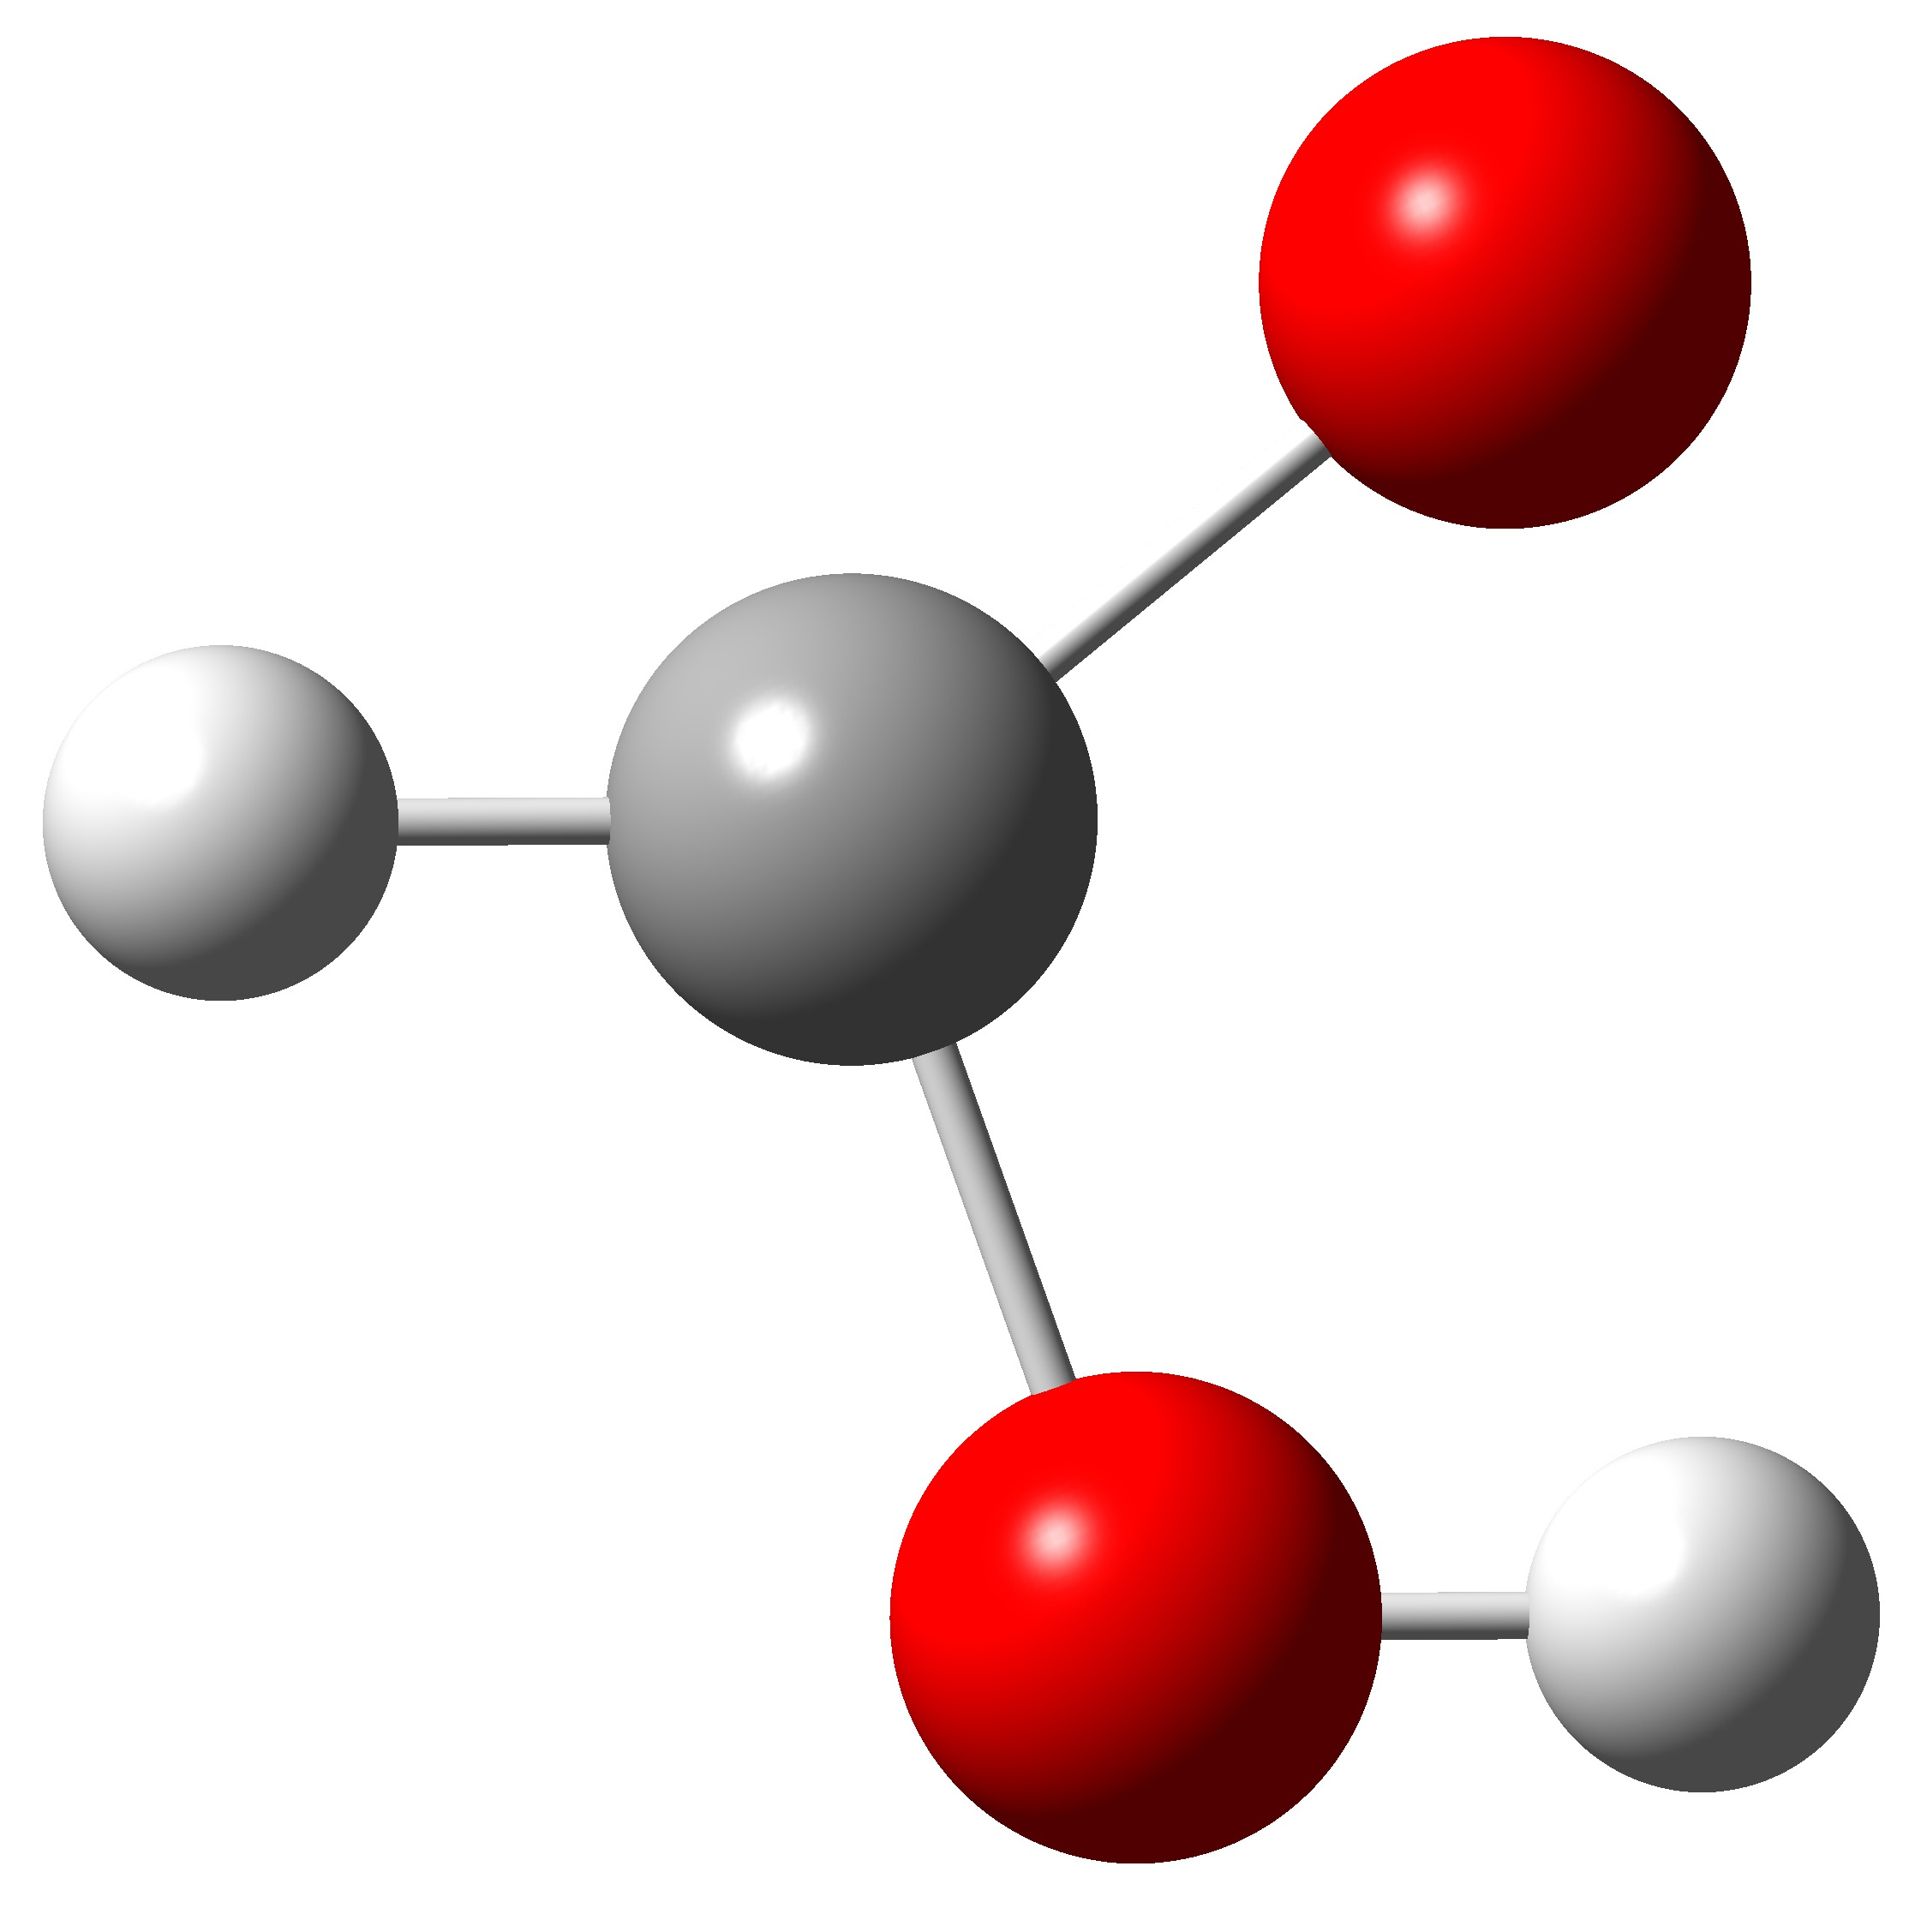
\includegraphics[scale=0.05]{formicAcid.jpg}
          \caption{Formic acid.}
        \end{minipage}
        \hfill
        \begin{minipage}[b]{0.225\textwidth}
          \centering
          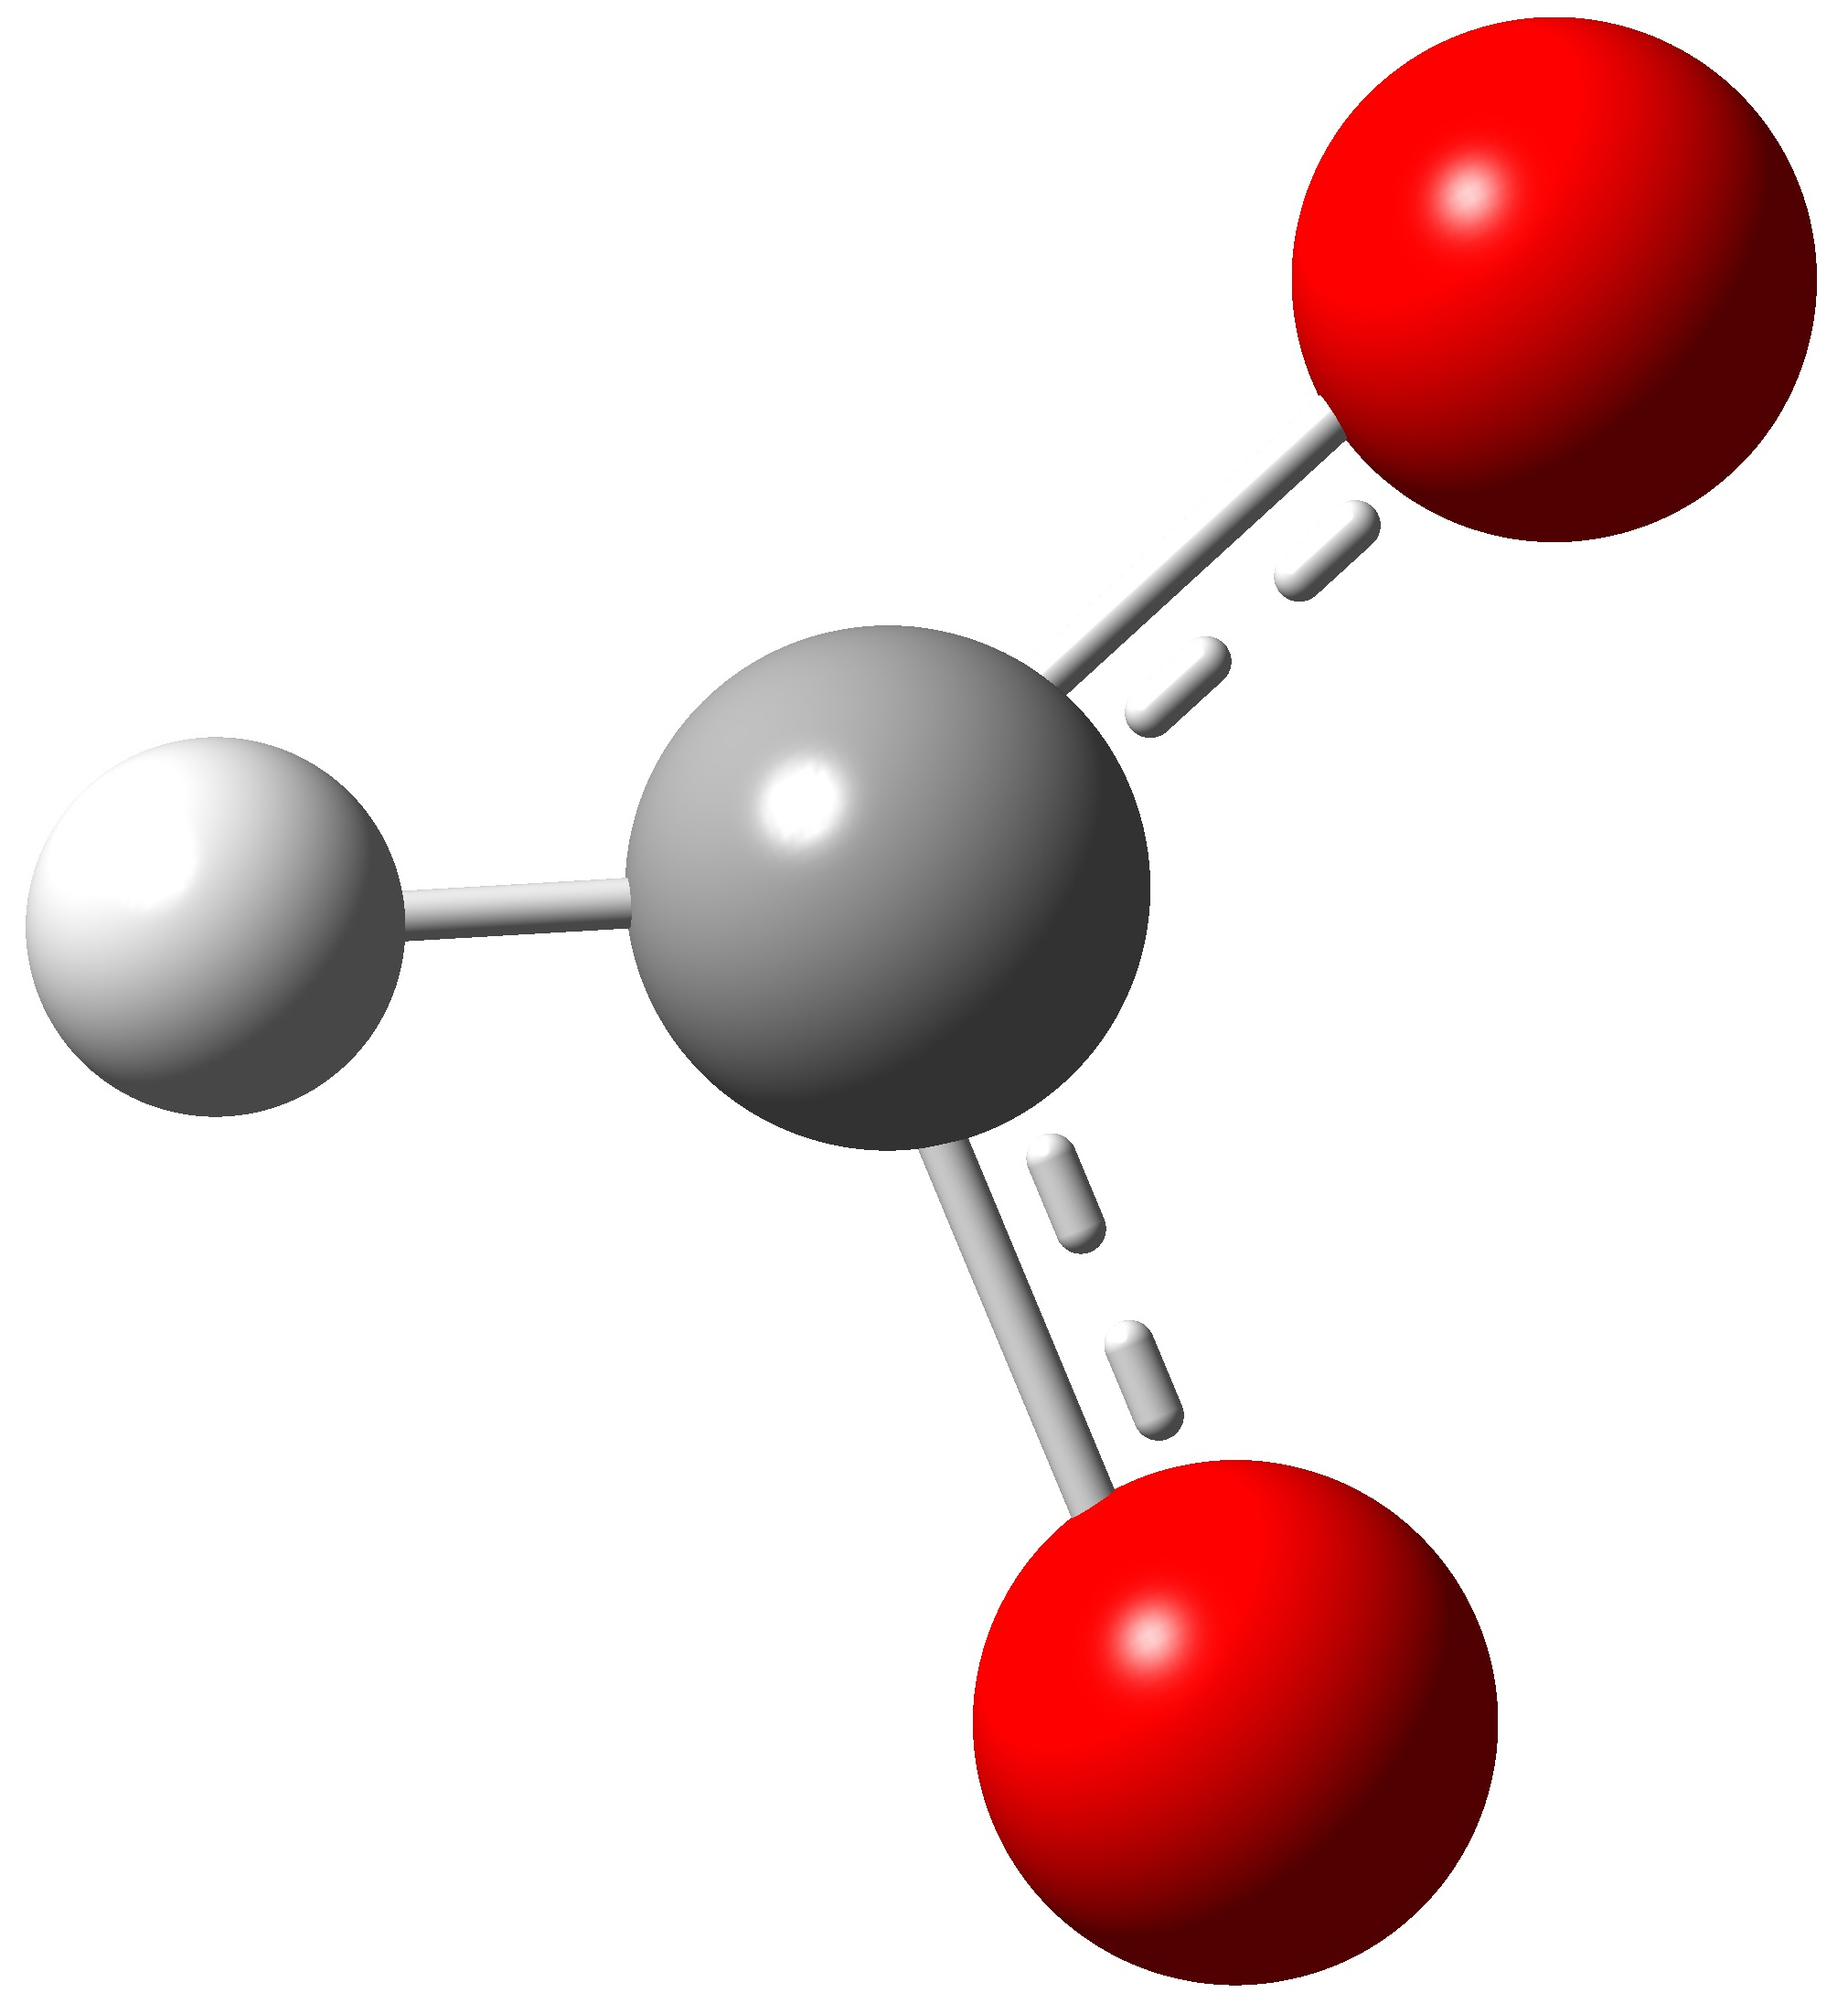
\includegraphics[scale=0.05]{formeate.jpg}
          \caption{Formiate anion.}
        \end{minipage}
        %water%
        \centering
        \begin{minipage}[b]{0.225\textwidth}
            \centering
          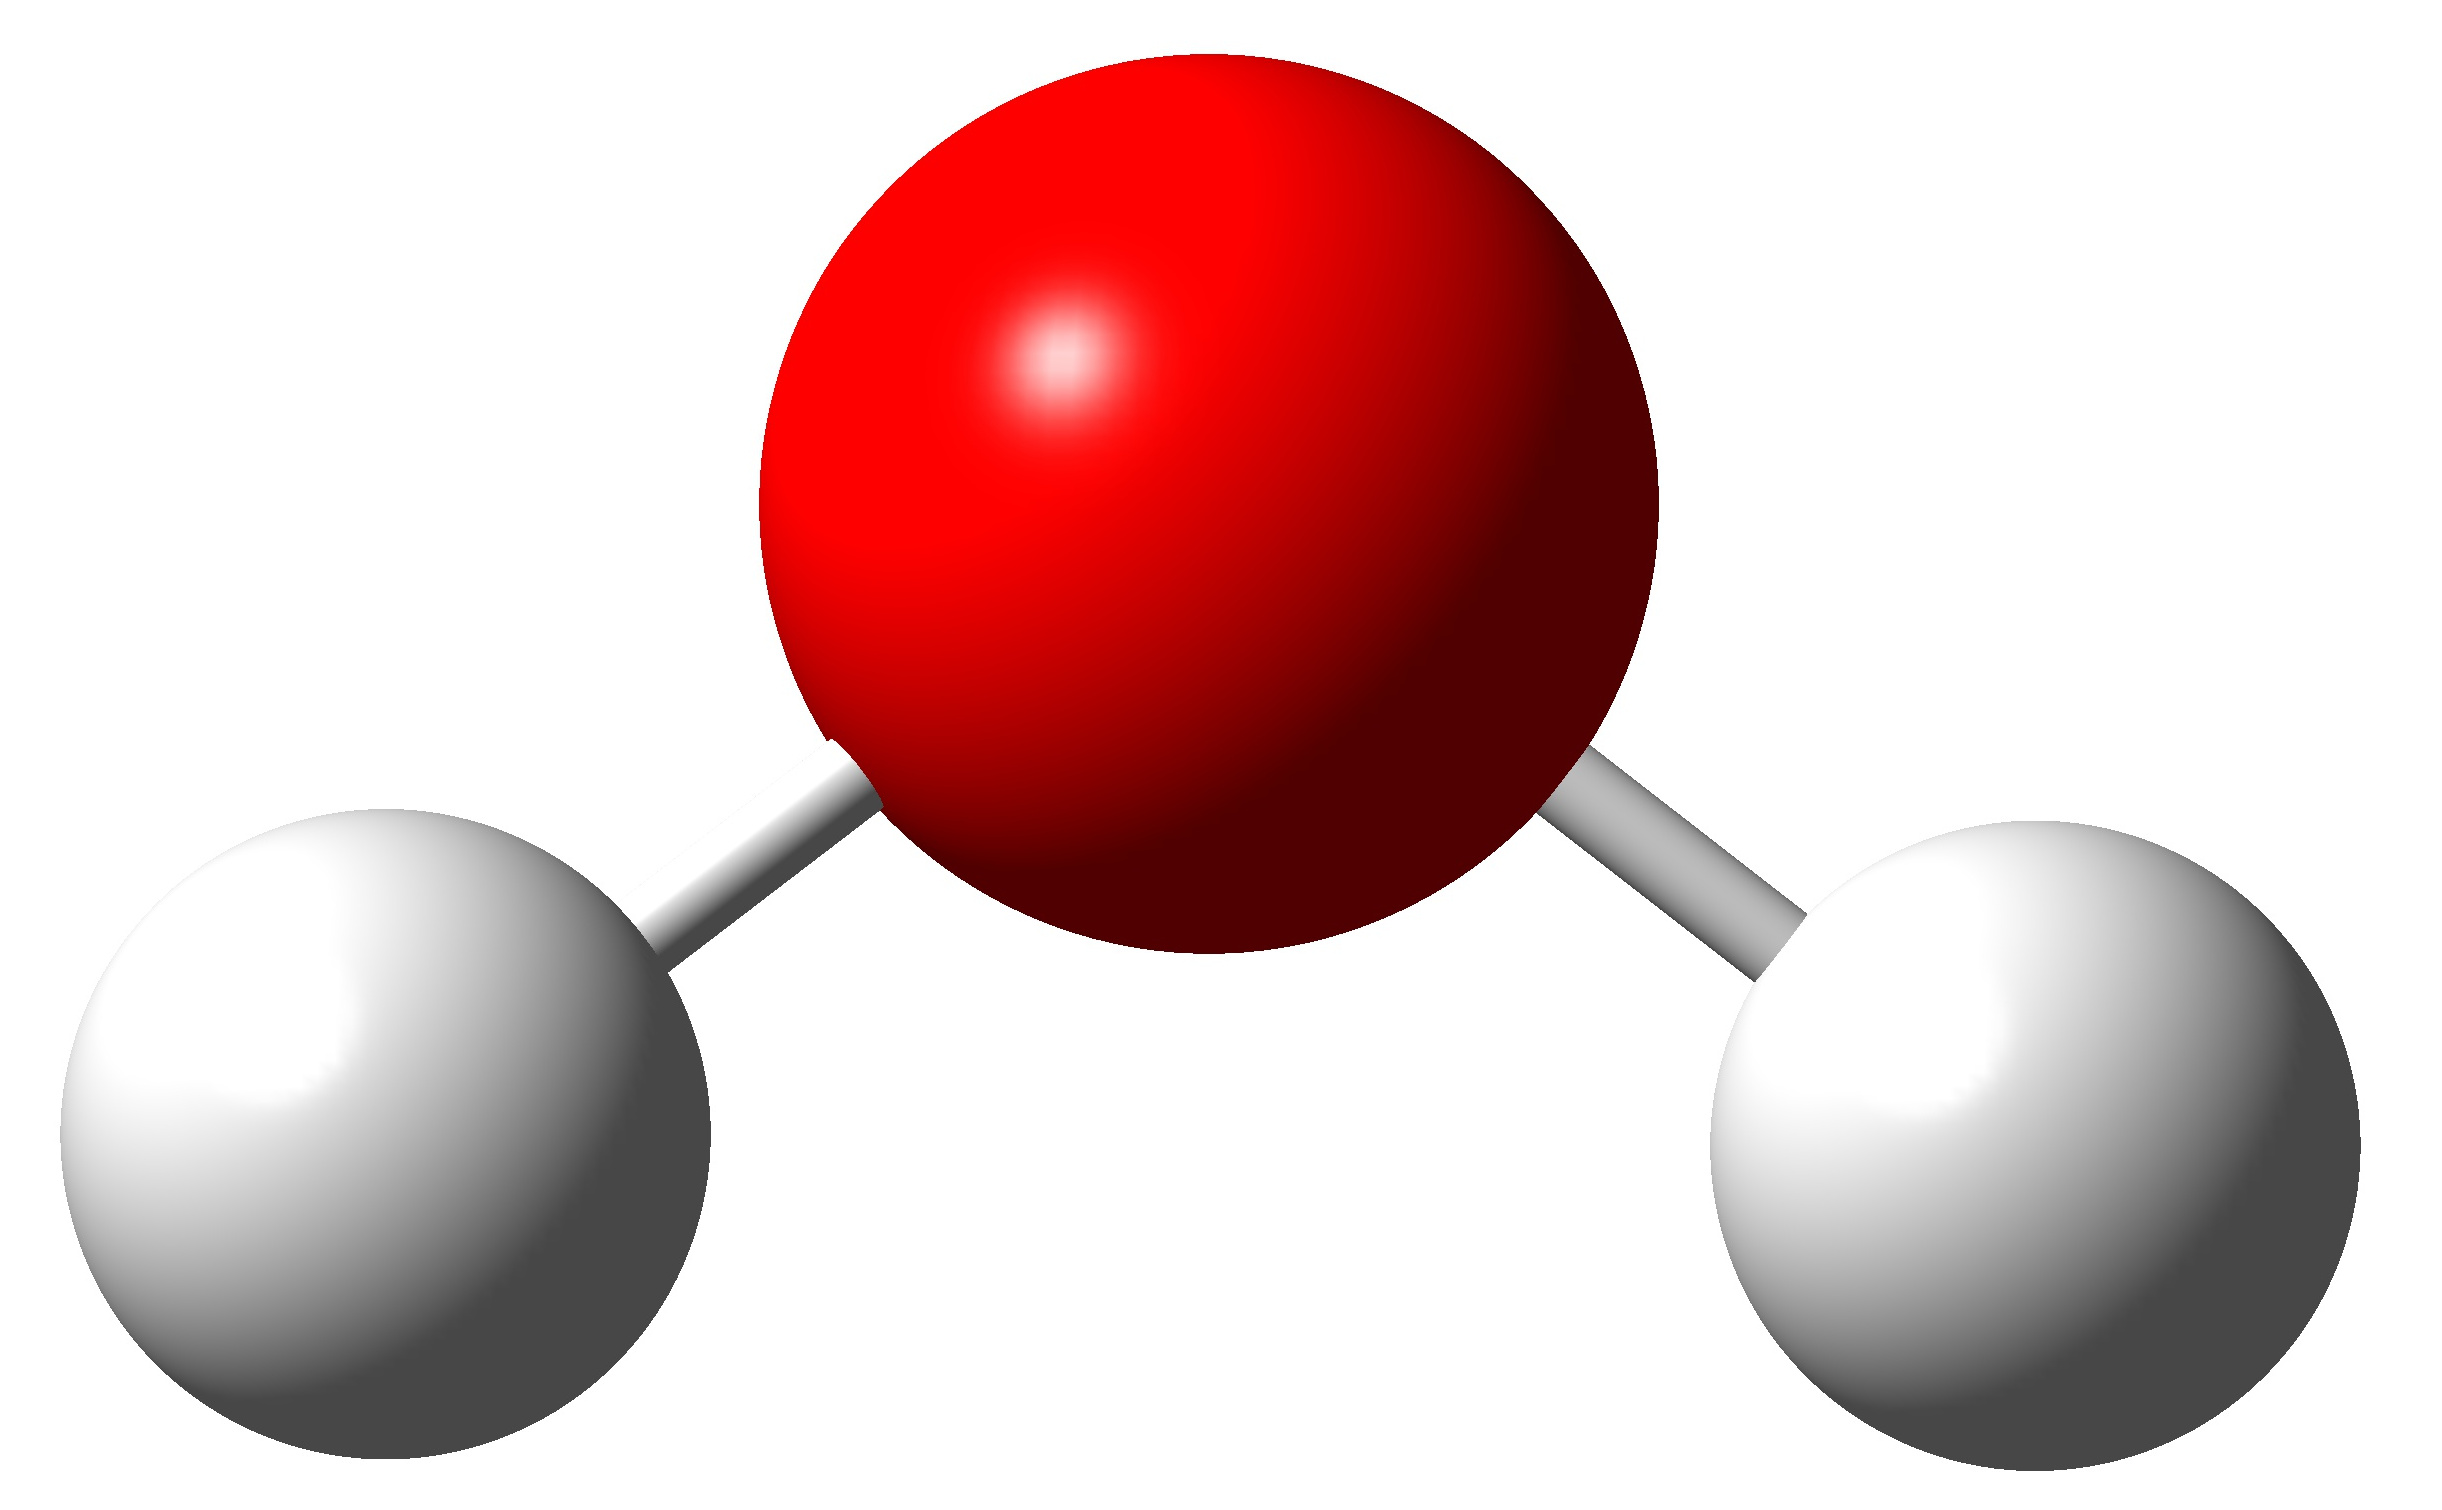
\includegraphics[scale=0.04]{water.jpg}
          \caption{Water.}
        \end{minipage}
        \hfill
        \begin{minipage}[b]{0.225\textwidth}
          \centering
          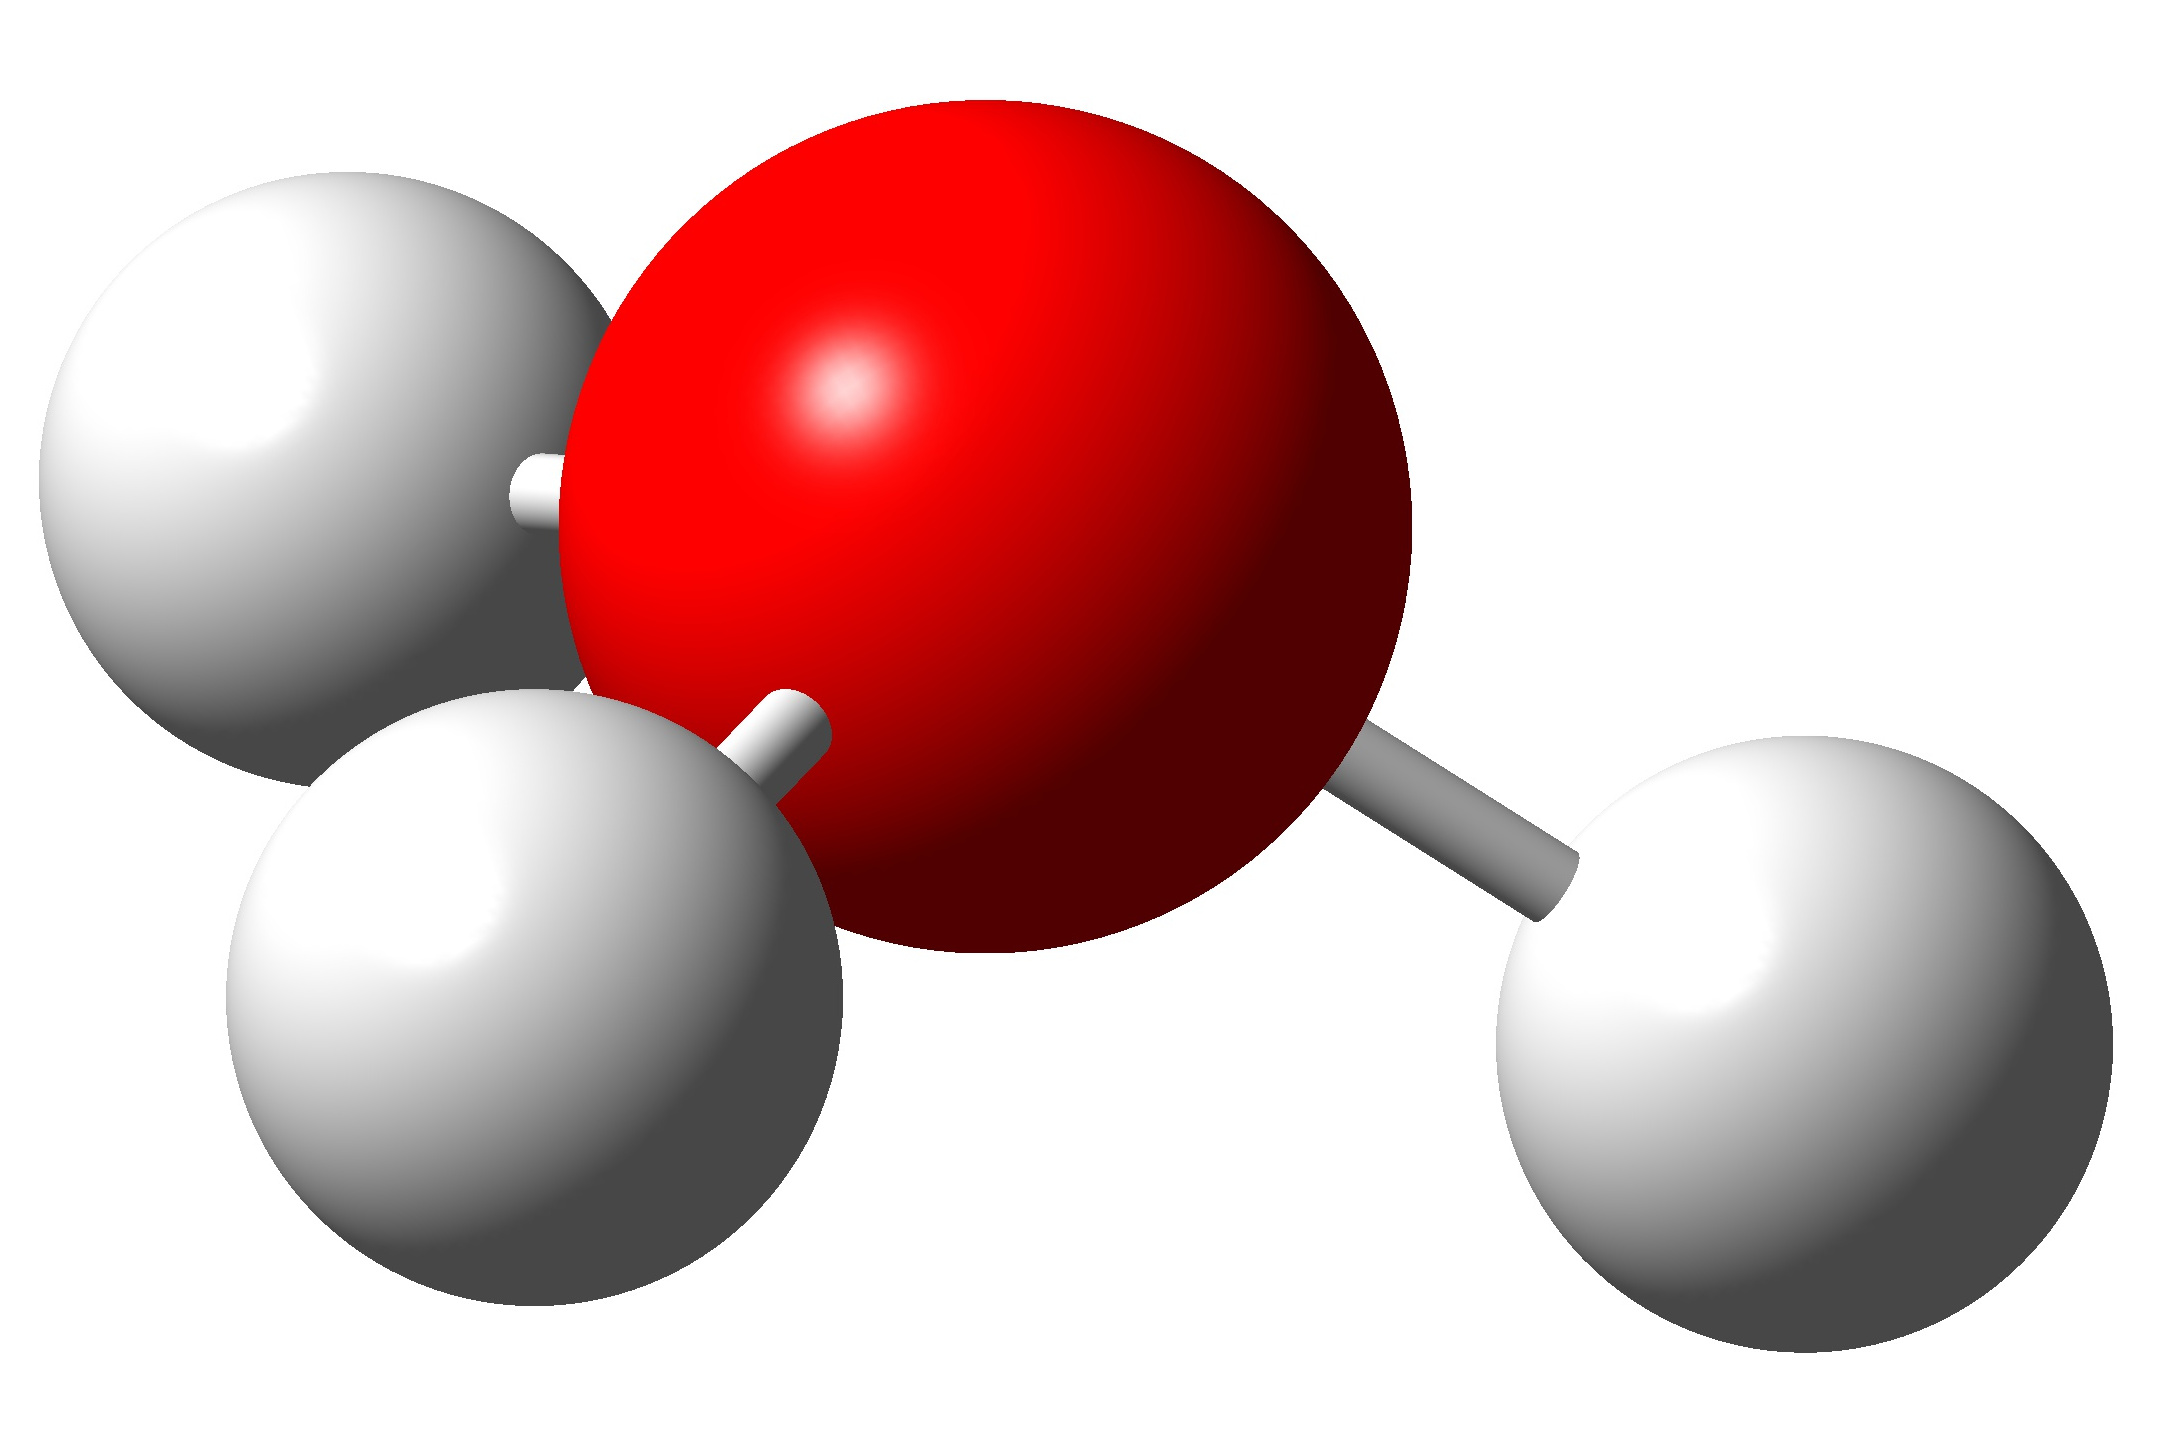
\includegraphics[scale=0.05]{hidronio.jpg}
          \caption{Hydronium.}
        \end{minipage}
        \centering
        \begin{minipage}[b]{0.225\textwidth}
            \centering
          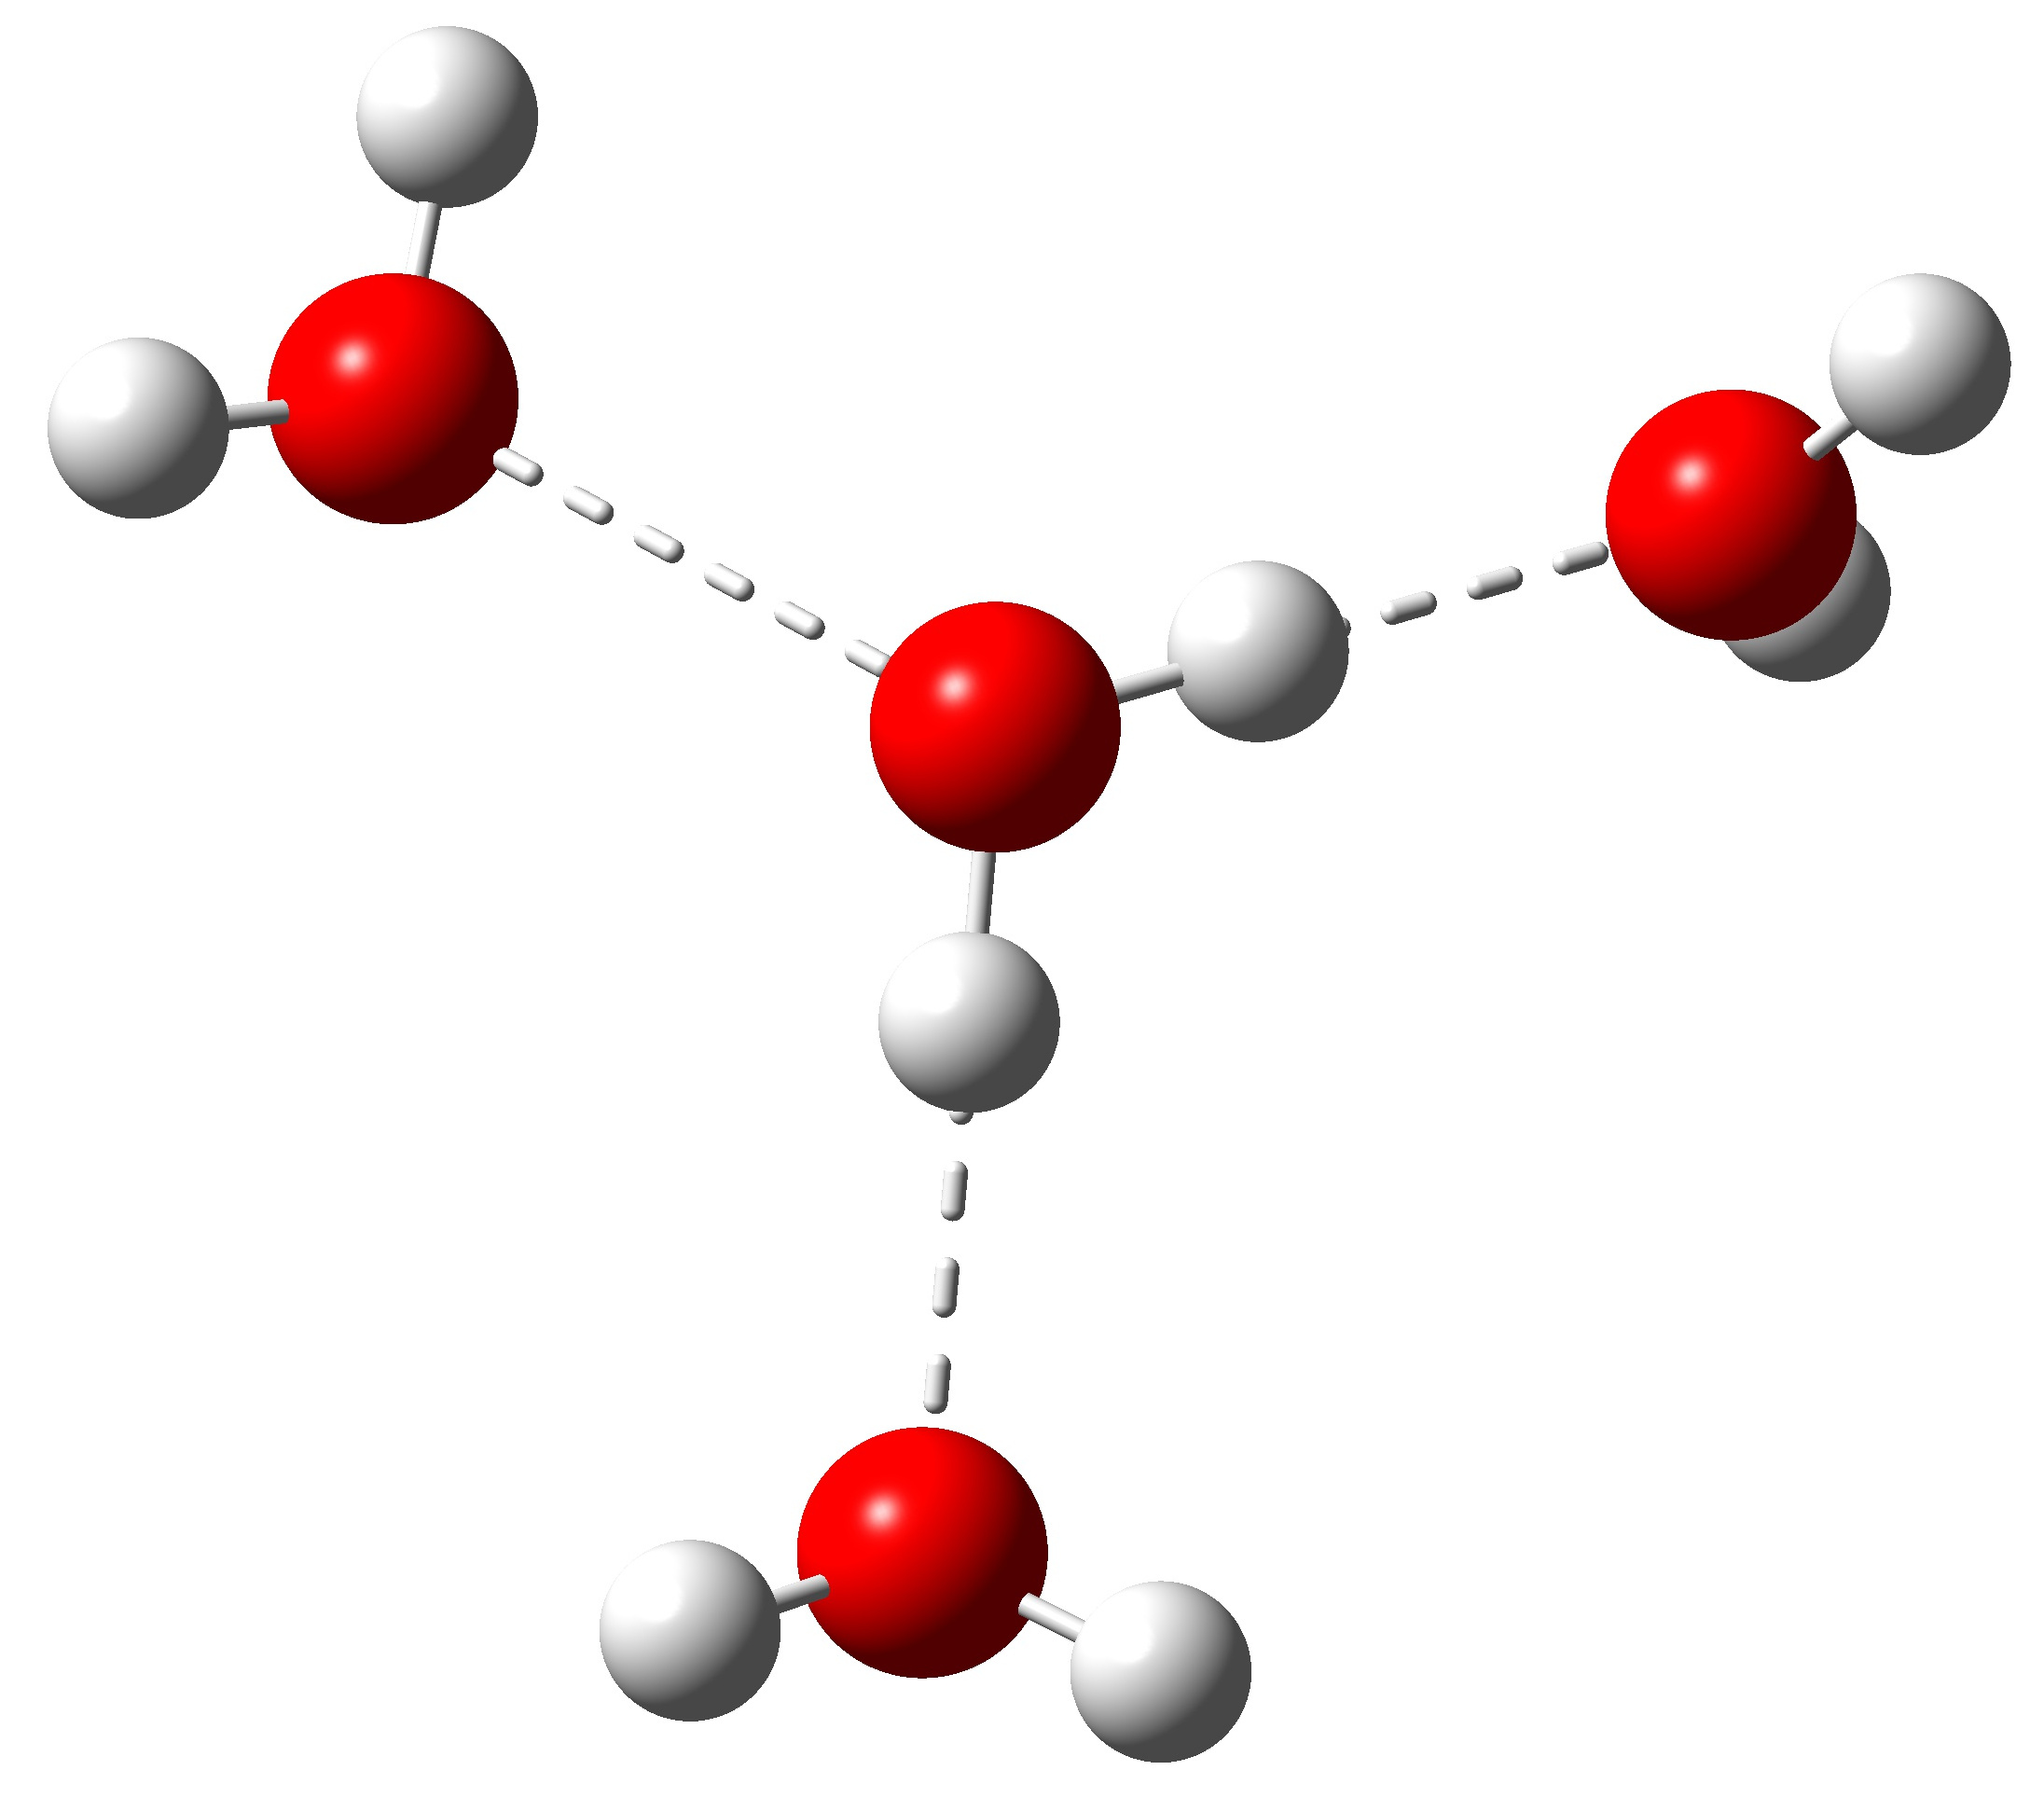
\includegraphics[scale=0.07]{4water.jpg}
          \caption{Water supermolecule.}
        \end{minipage}
        \hfill
        \begin{minipage}[b]{0.225\textwidth}
          \centering
          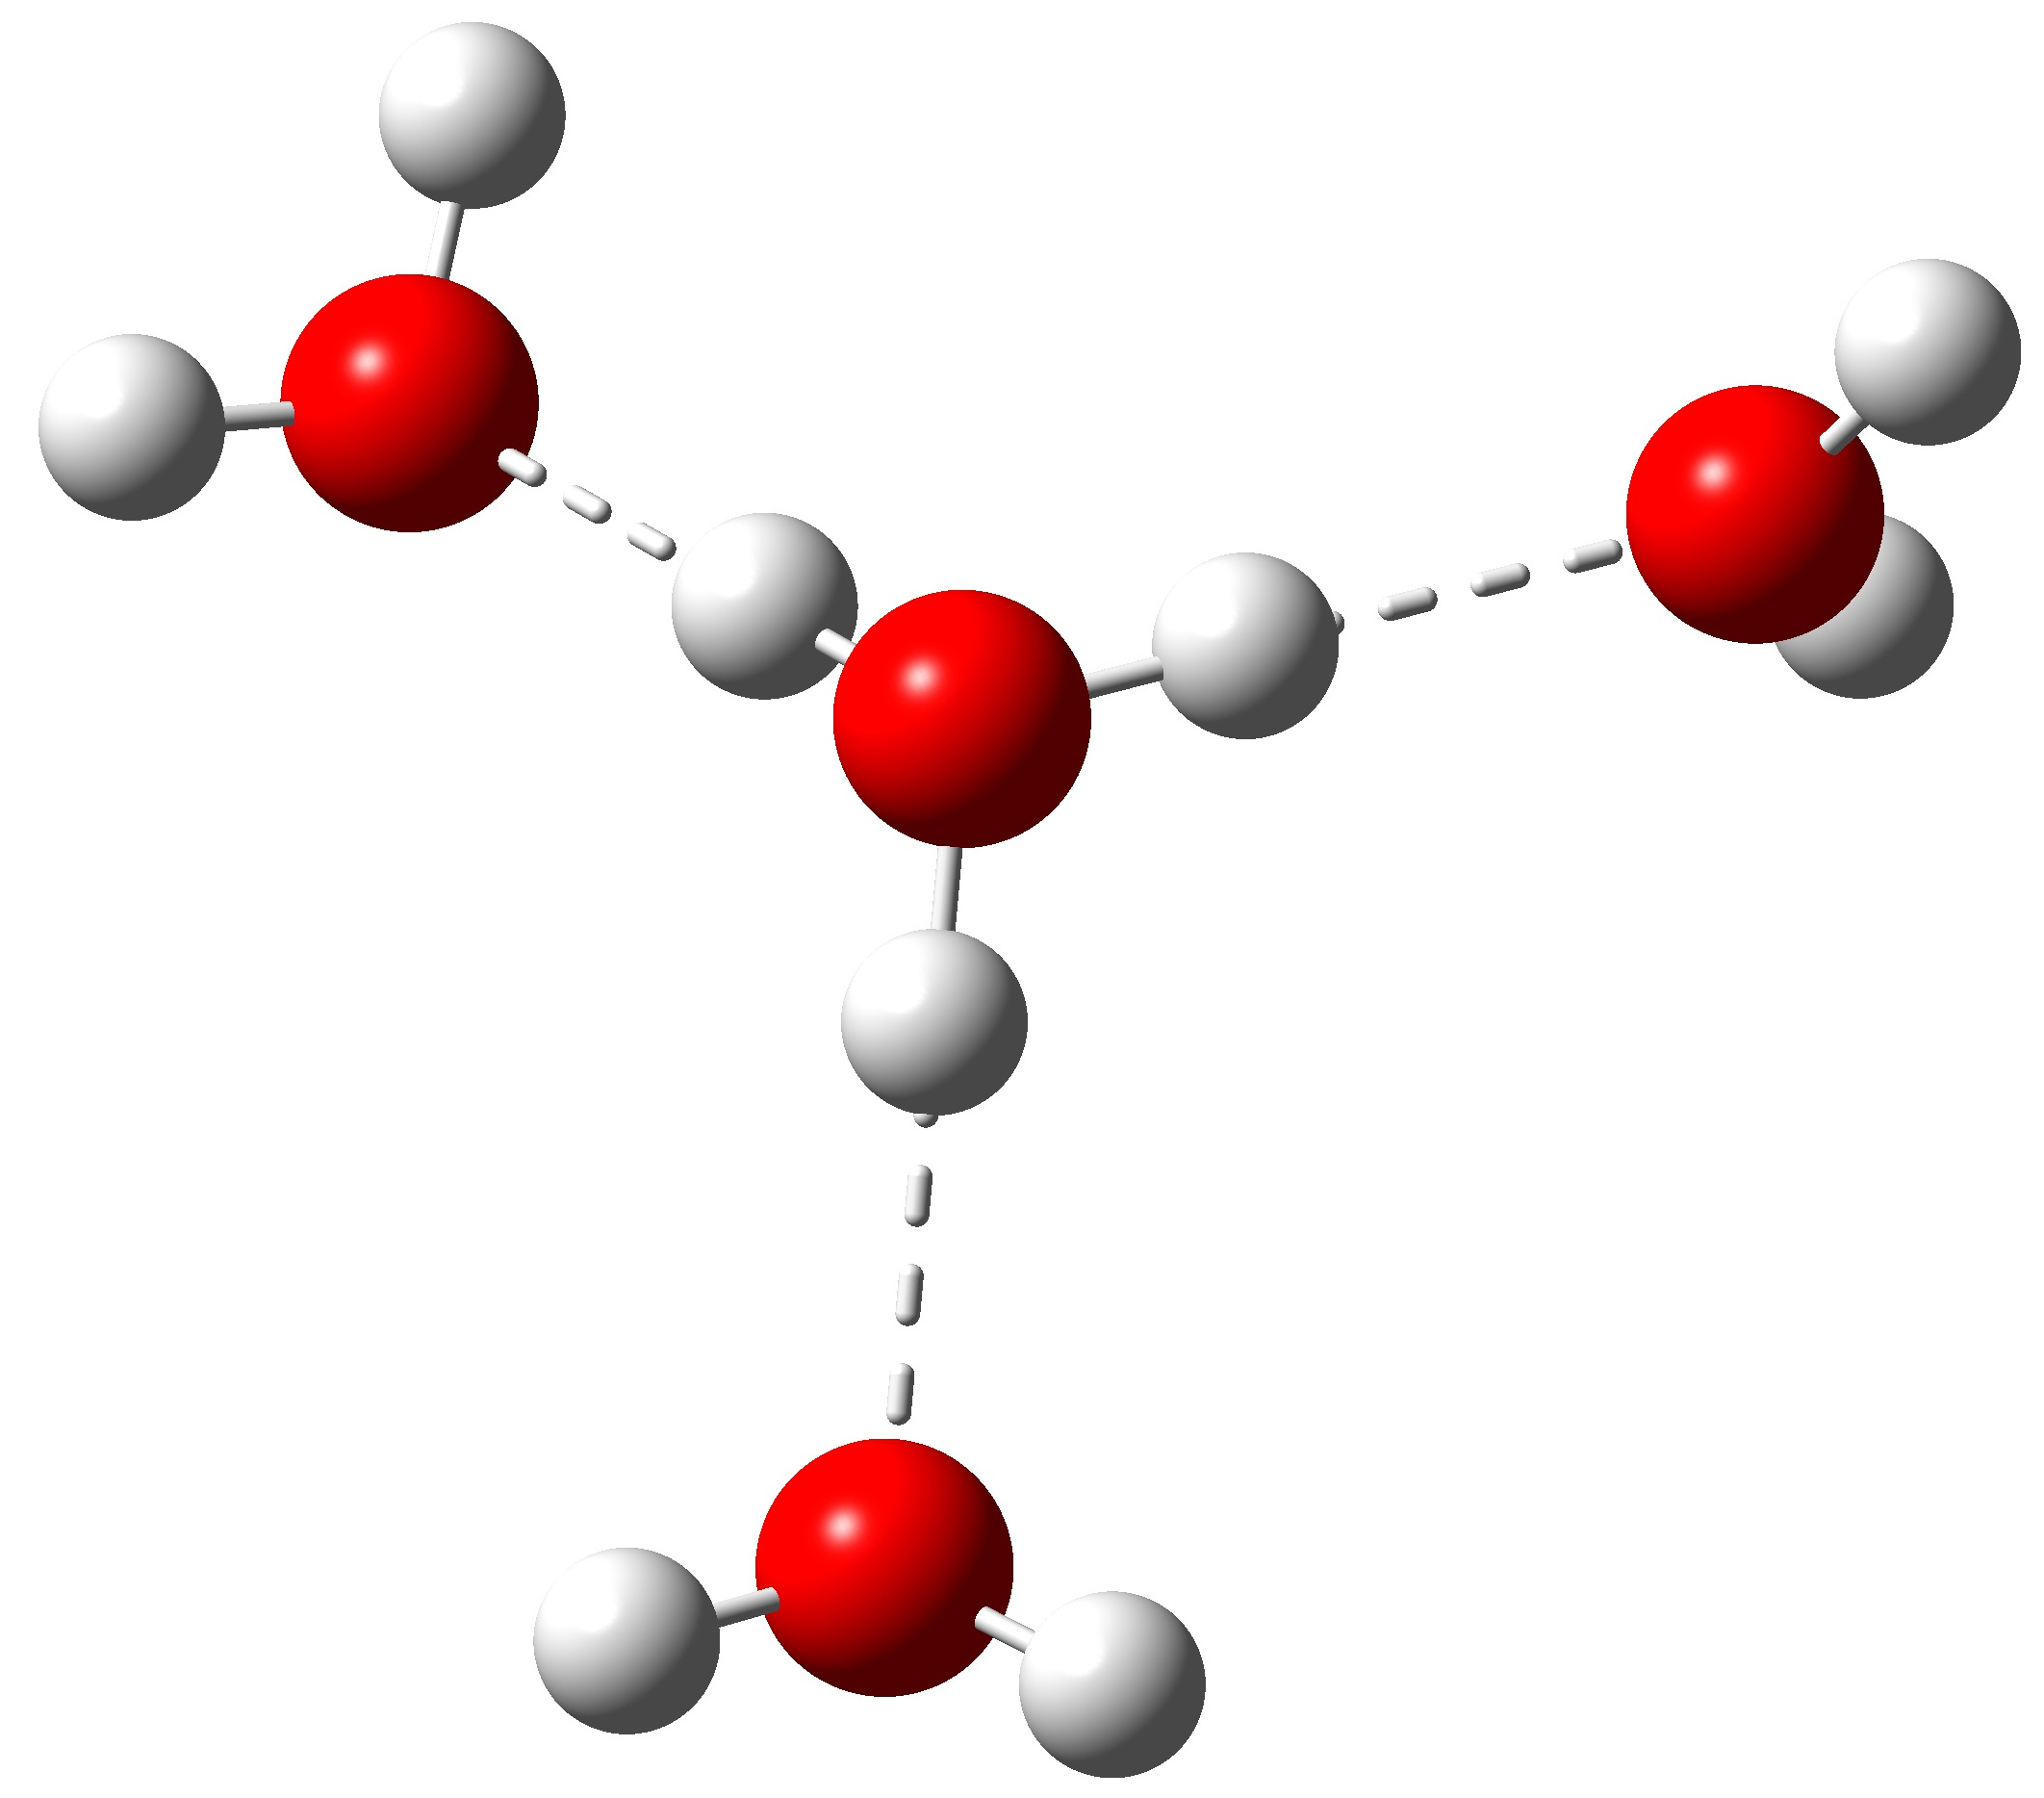
\includegraphics[scale=0.08]{hidronio4waters.jpg}
          \caption{Hydronium supermolecule.}
        \end{minipage}
        \centering
        \begin{minipage}[b]{0.225\textwidth}
            \centering
          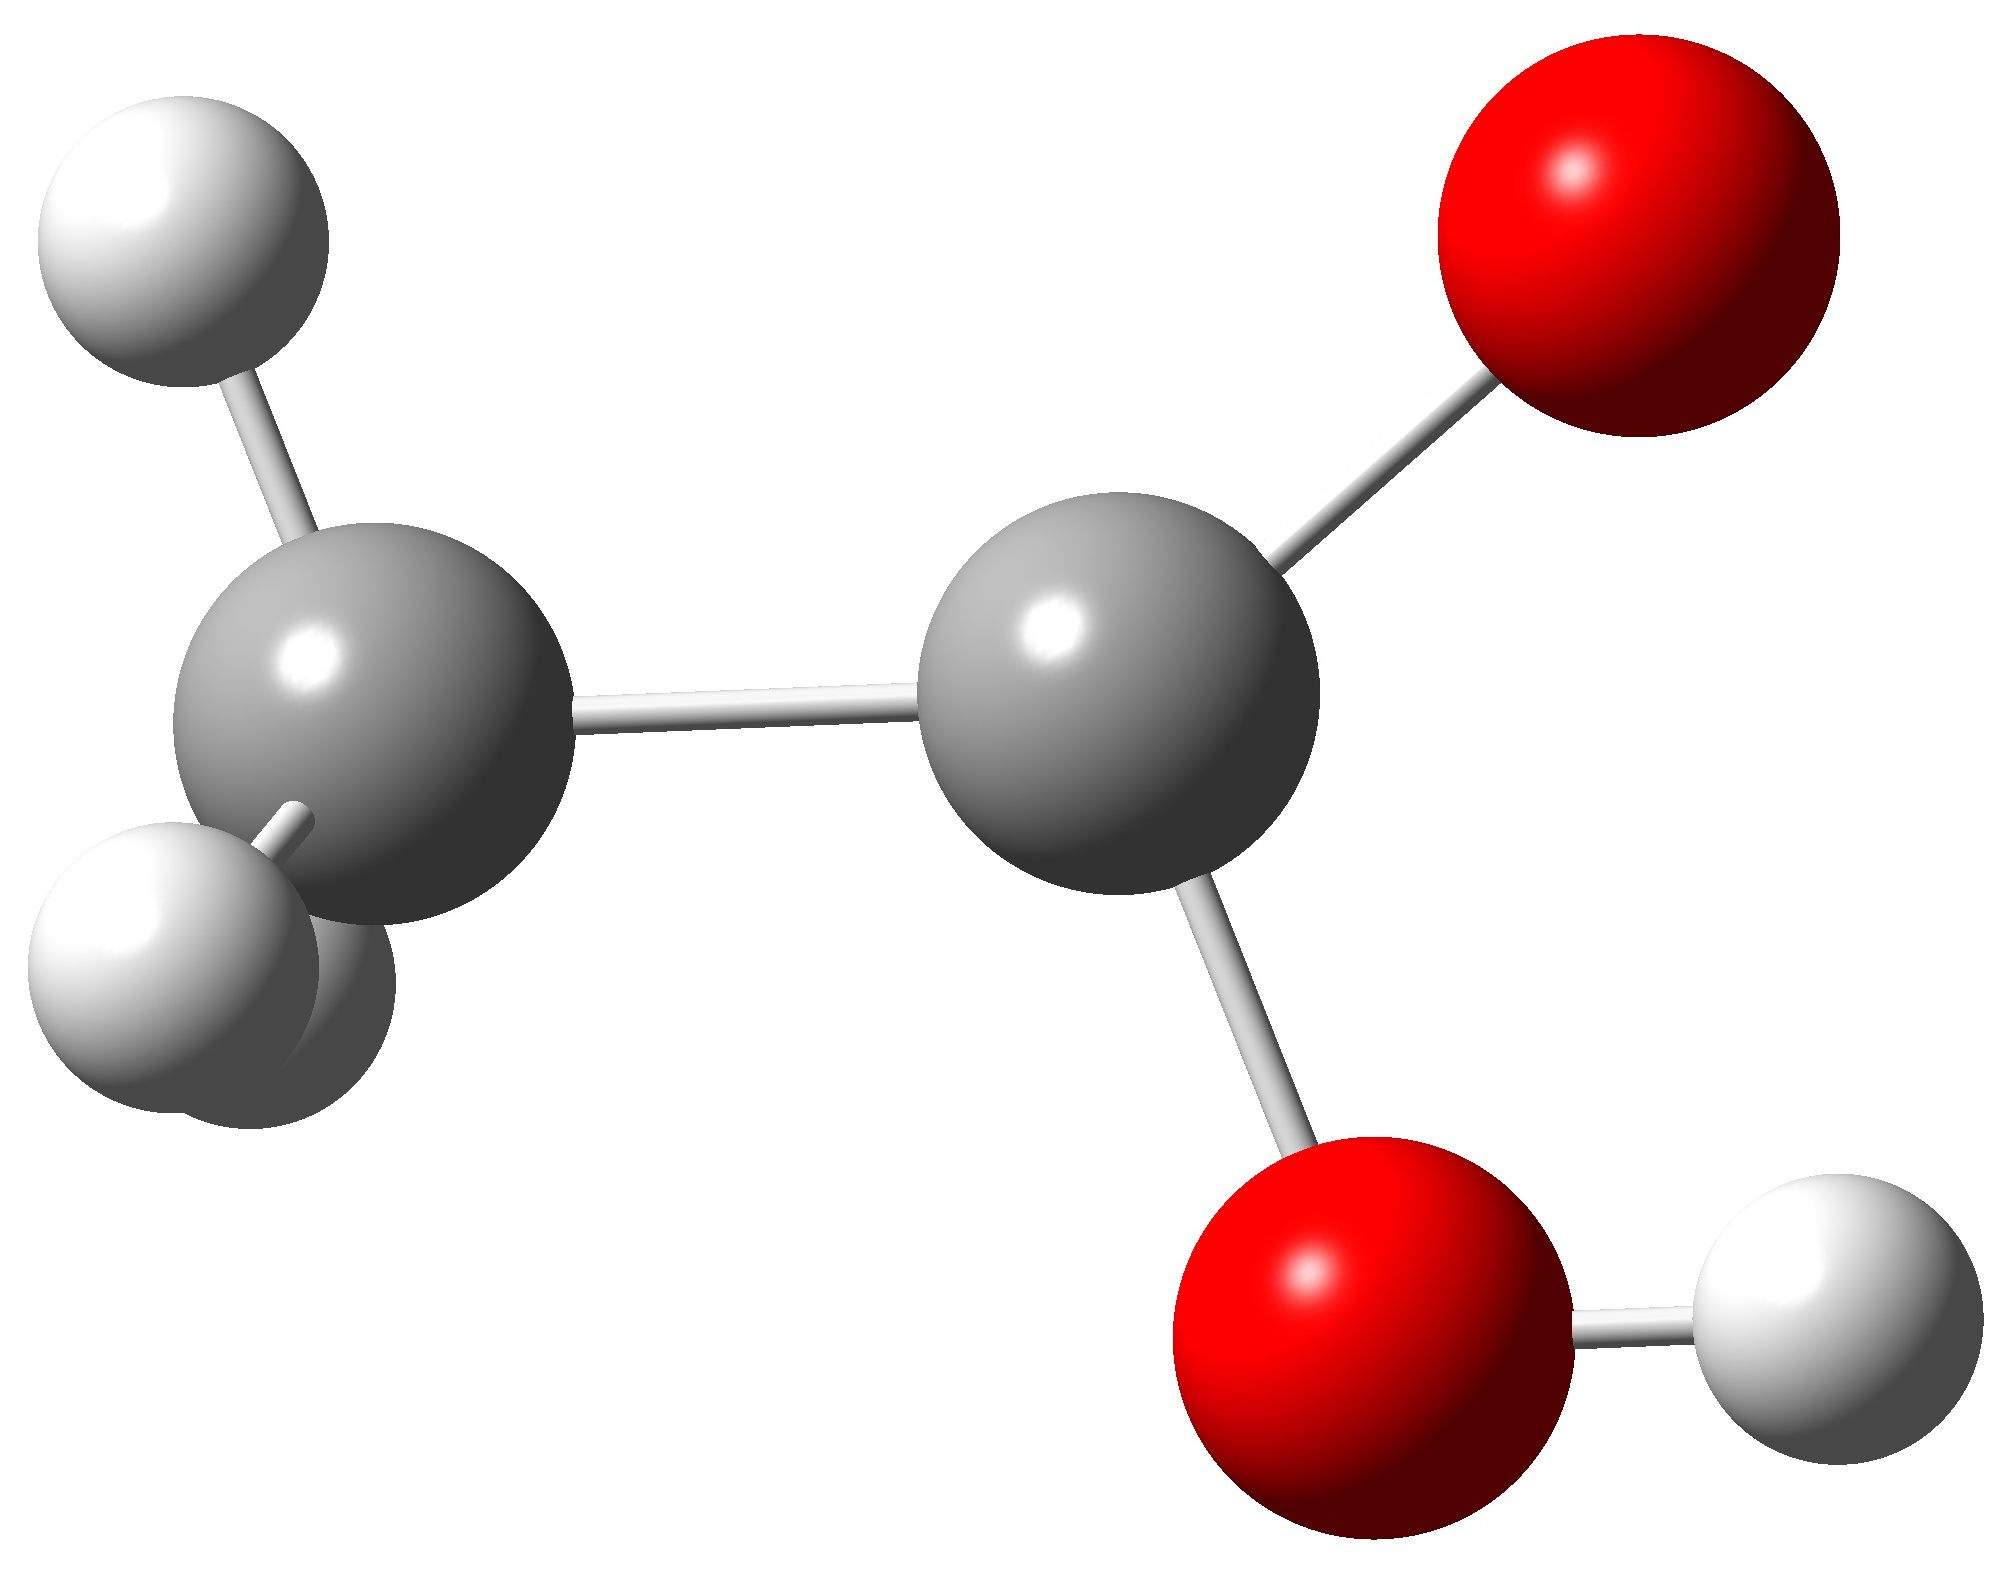
\includegraphics[scale=0.07]{aceticAcid.jpg}
          \caption{Acetic acid.}
        \end{minipage}
        \hfill
        \begin{minipage}[b]{0.225\textwidth}
          \centering
          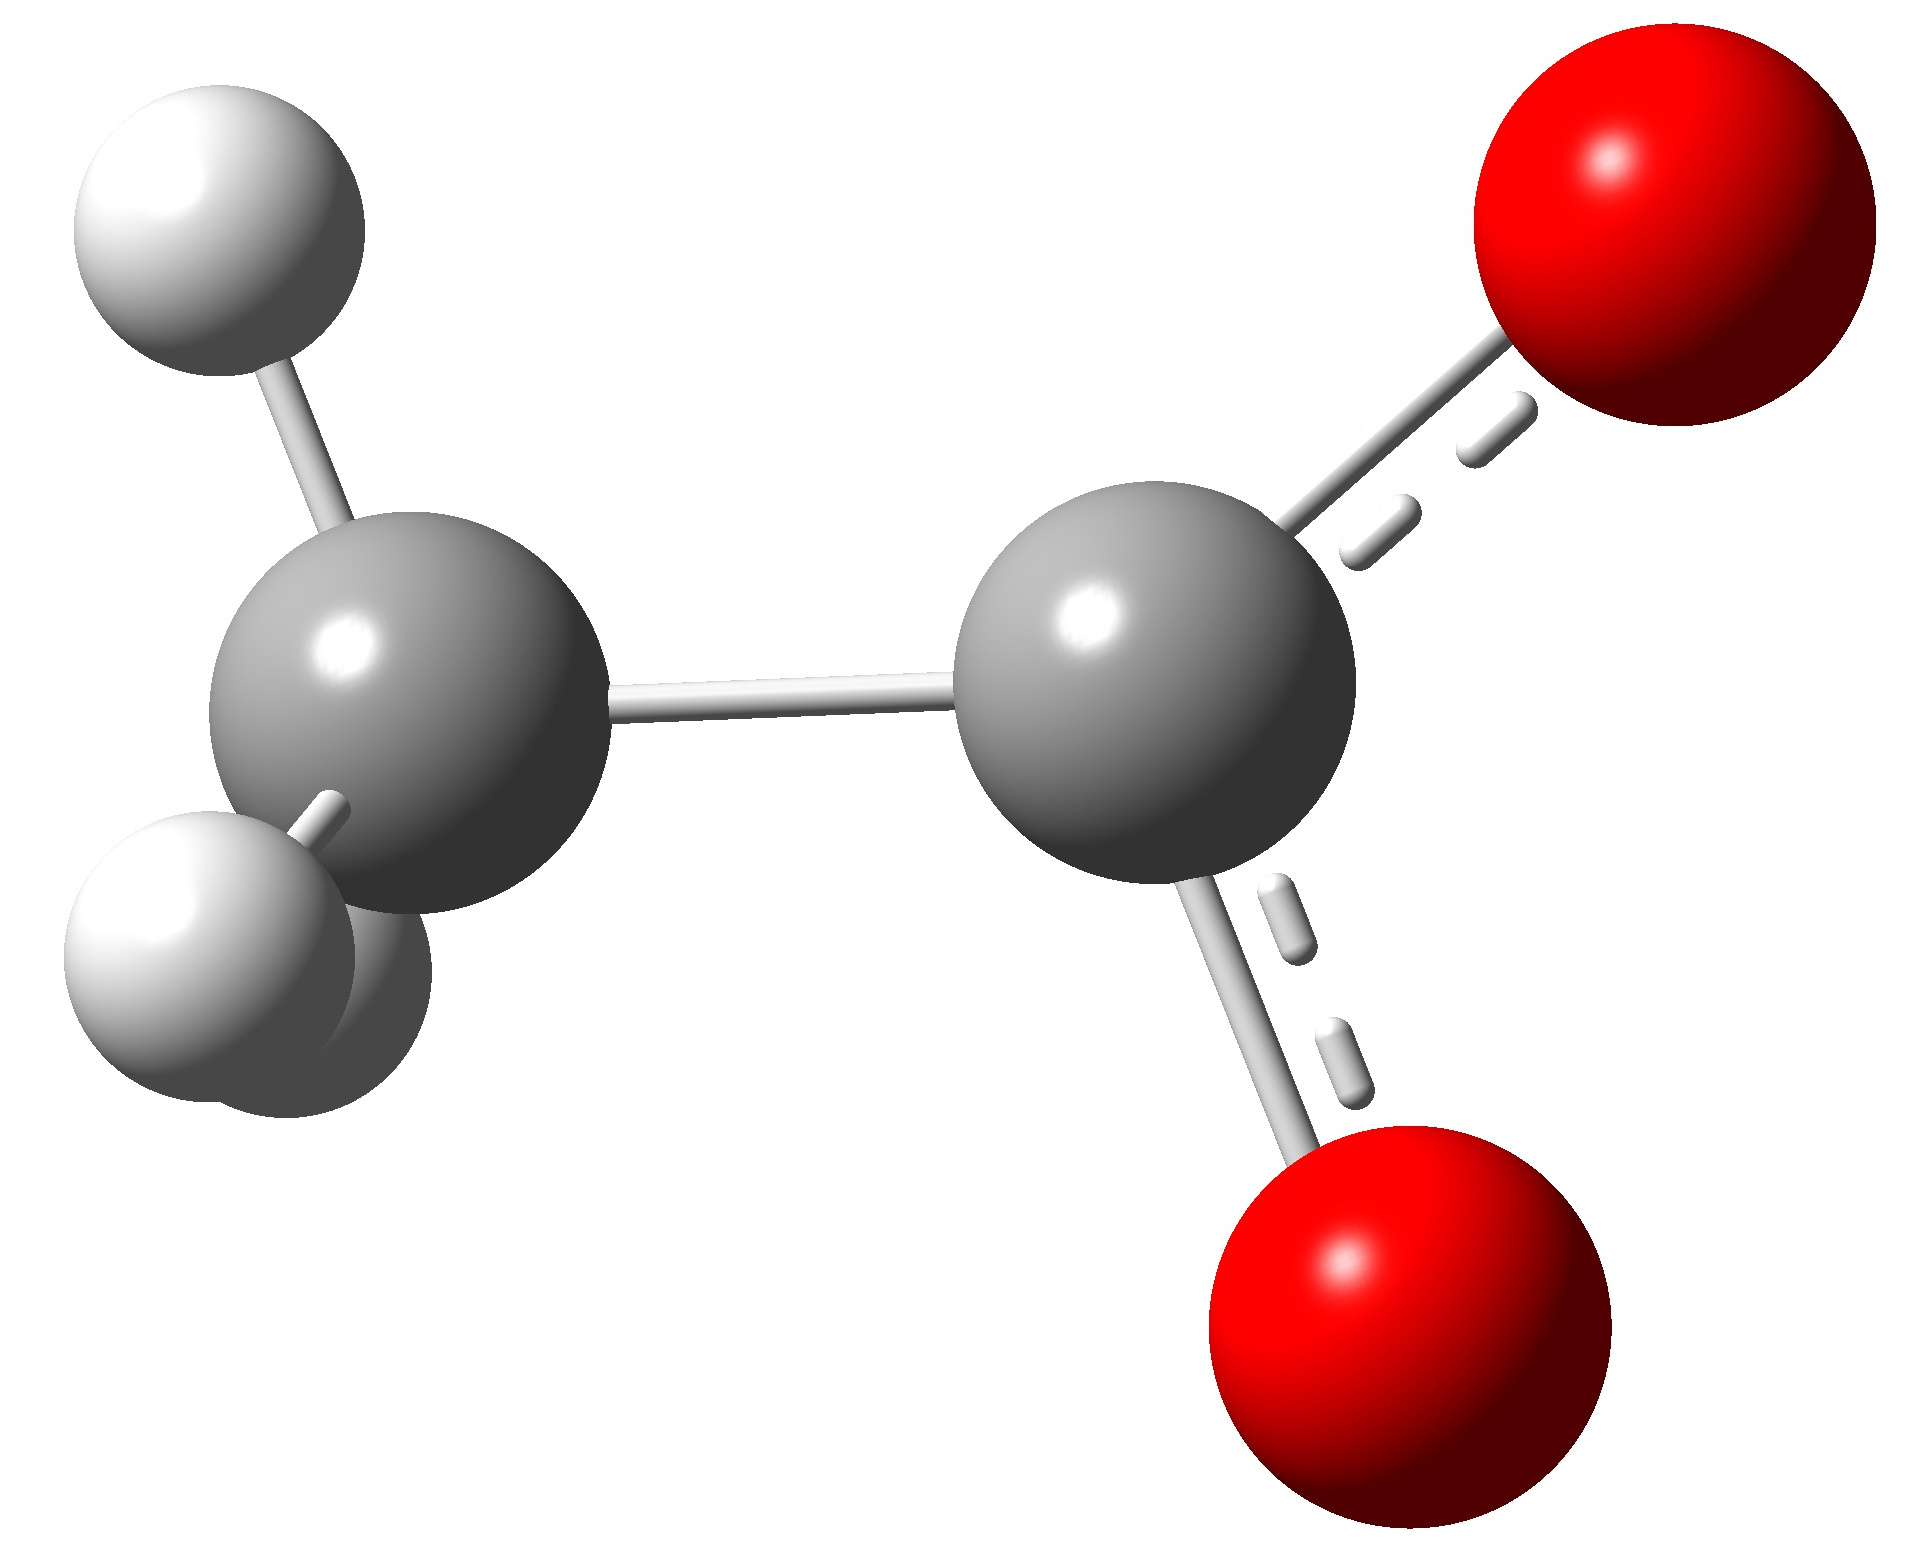
\includegraphics[scale=0.08]{acetate.jpg}
          \caption{Acetate anion.}
        \end{minipage}
        \centering
        \begin{minipage}[b]{0.225\textwidth}
            \centering
          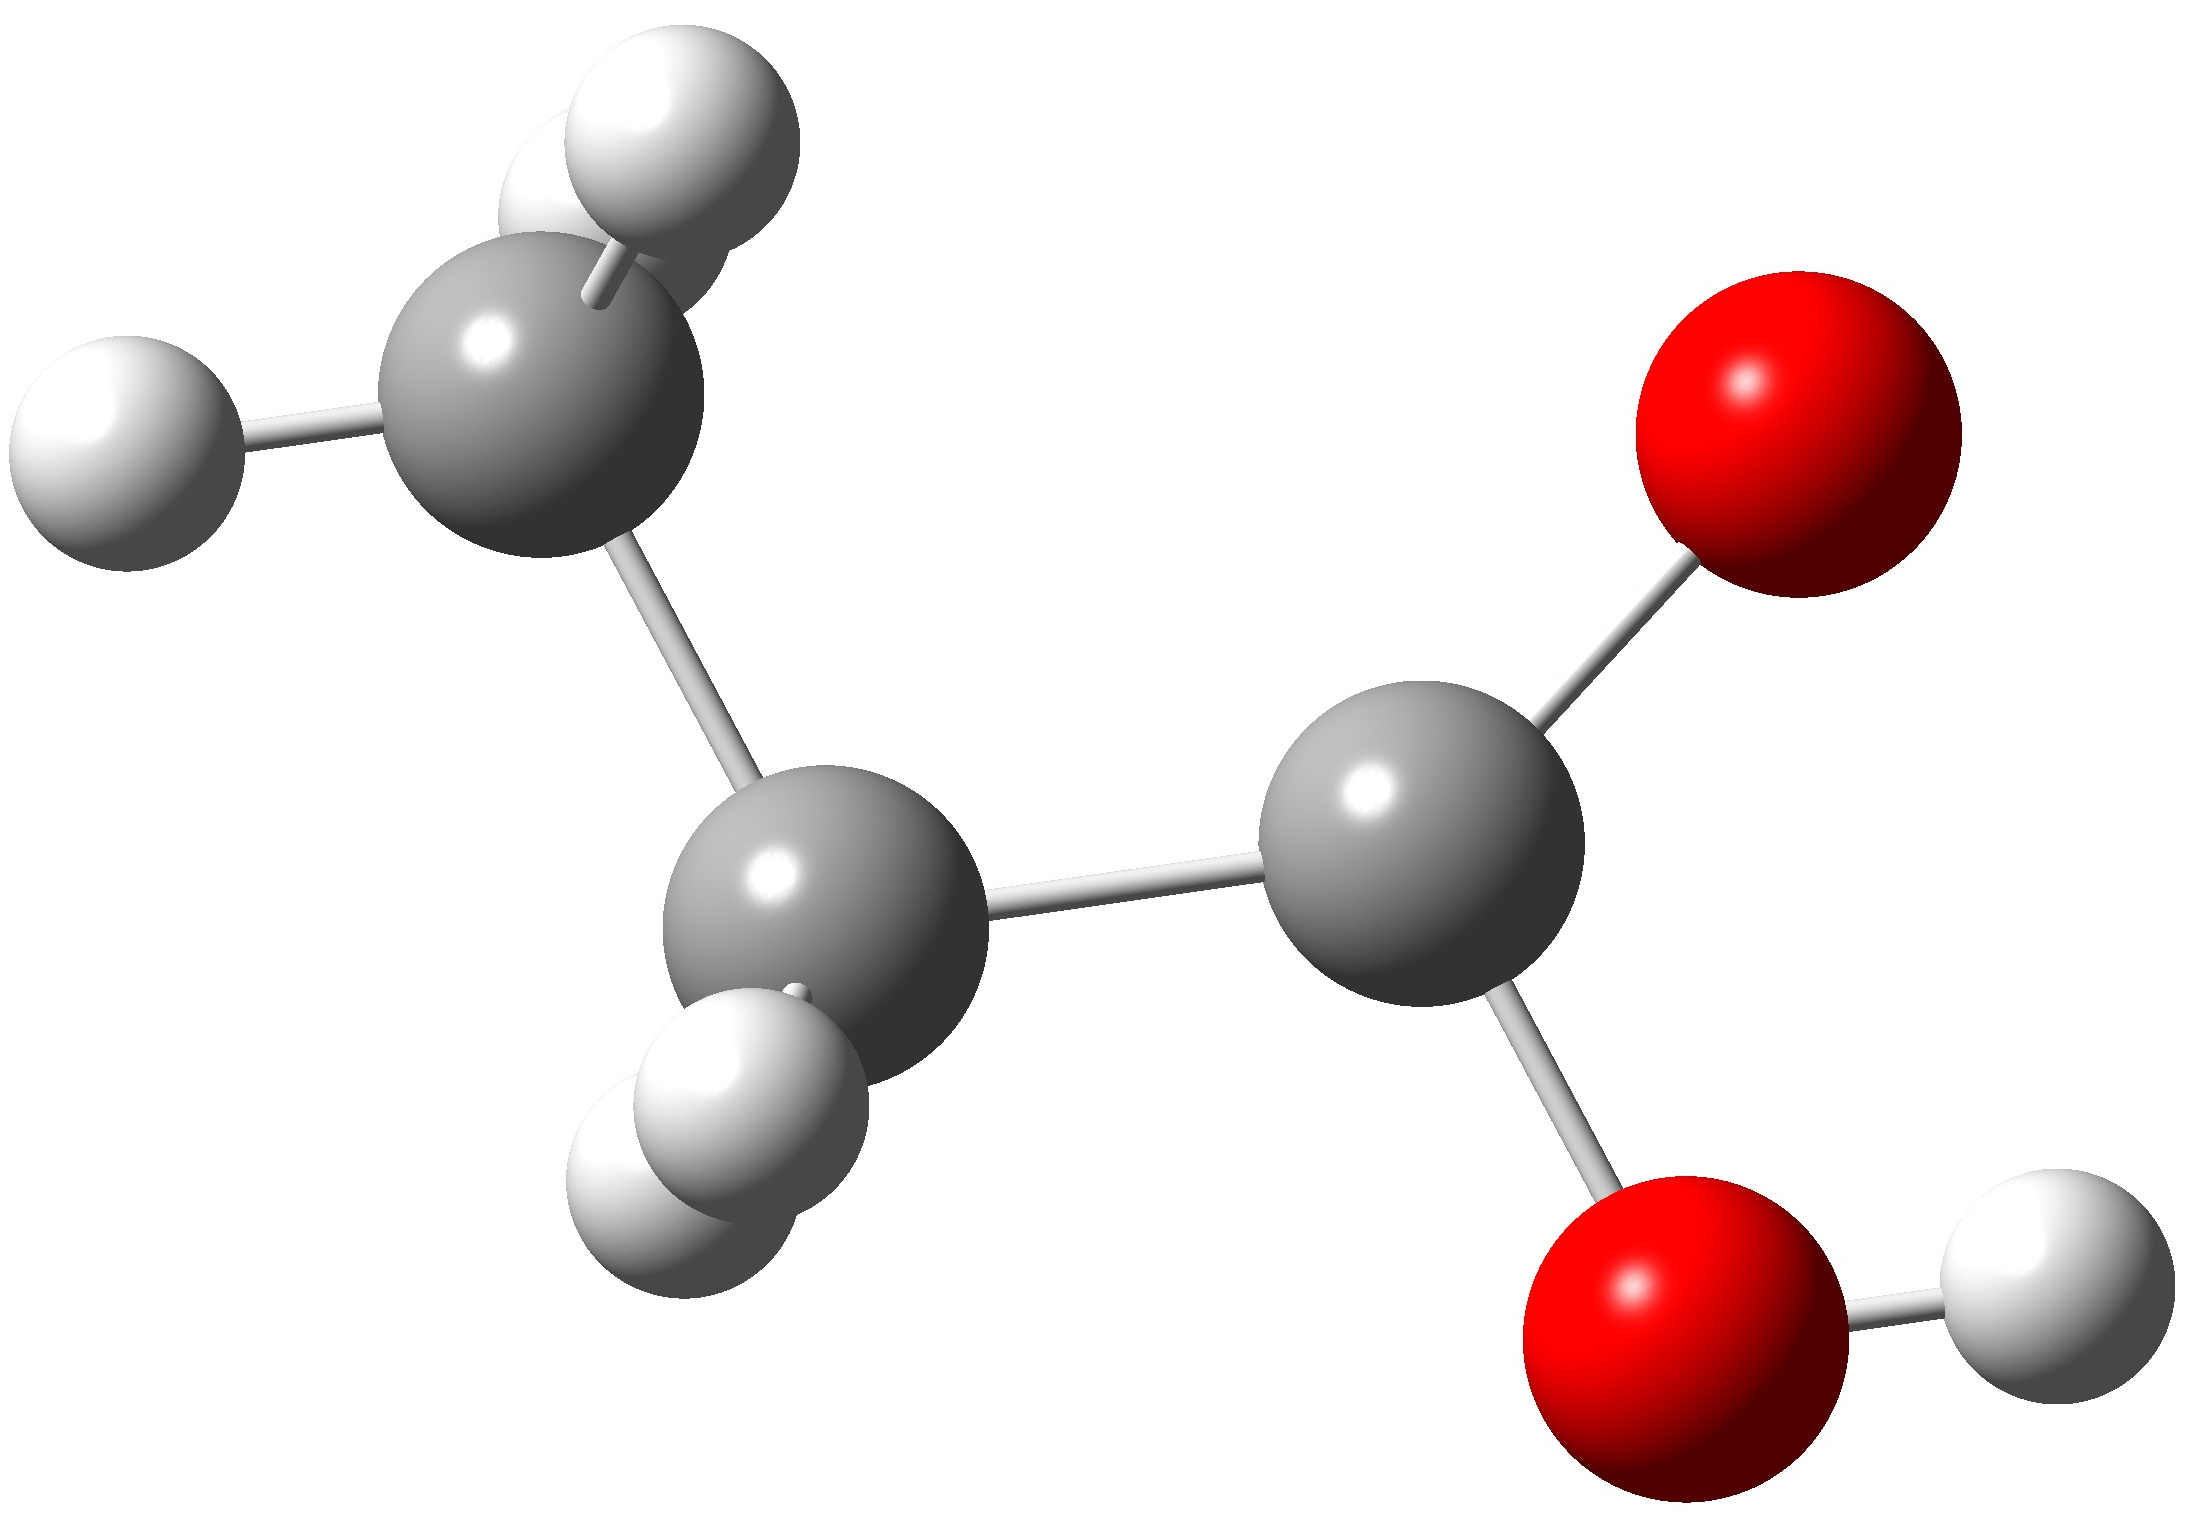
\includegraphics[scale=0.07]{propanoicAcid.jpg}
          \caption{Propanoic acid.}
        \end{minipage}
        \hfill
        \begin{minipage}[b]{0.225\textwidth}
          \centering
          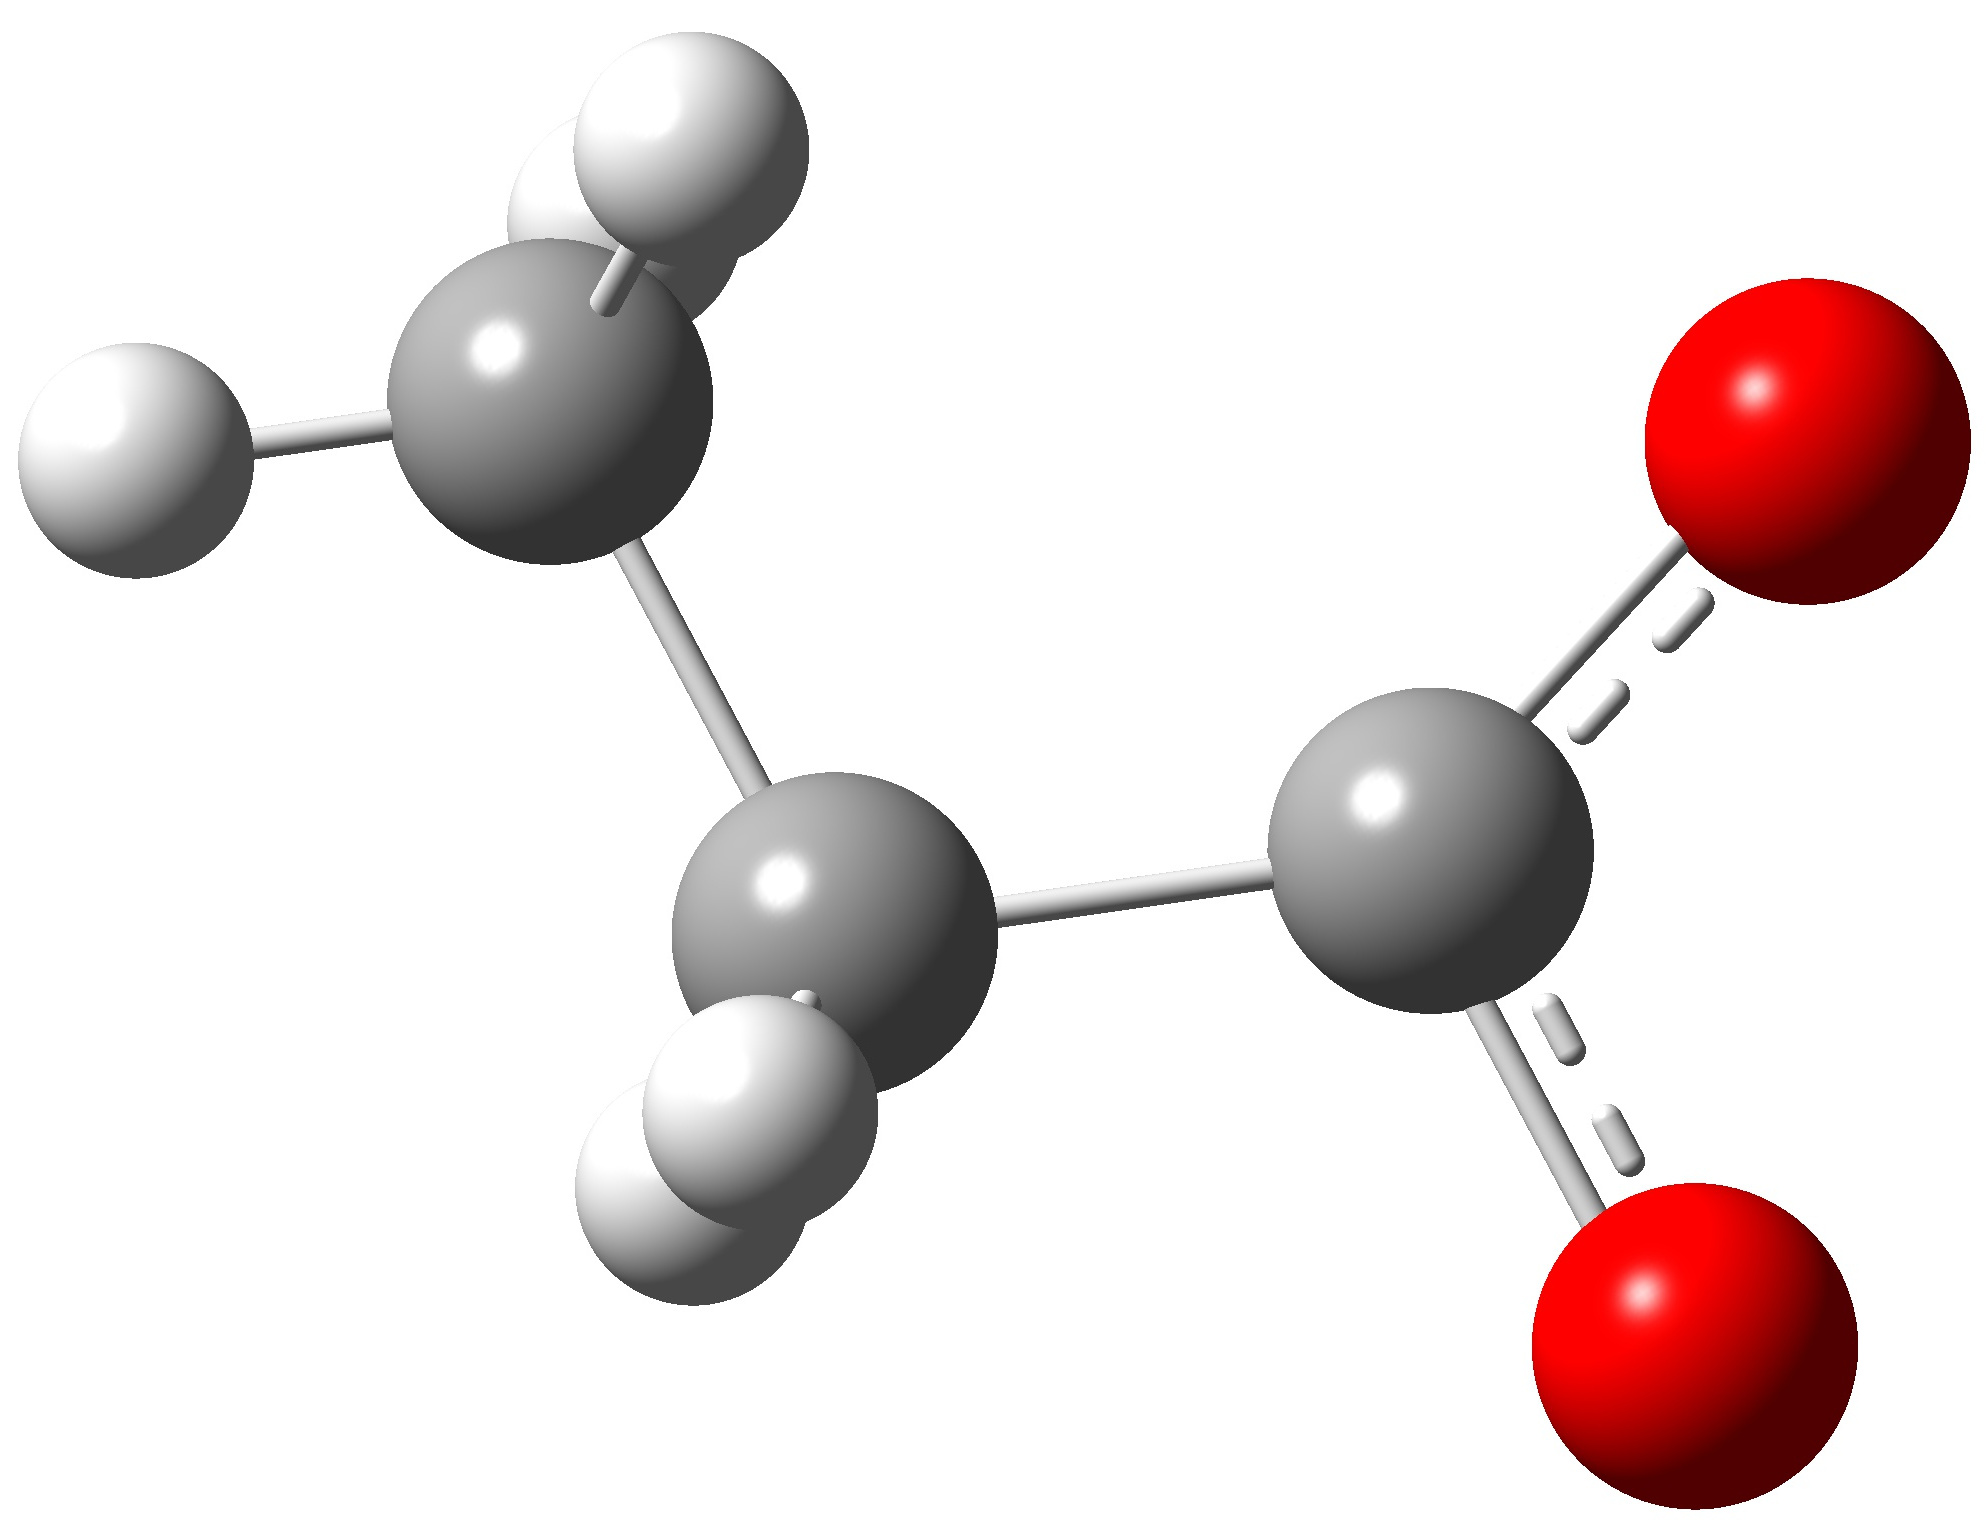
\includegraphics[scale=0.08]{propanoate.jpg}
          \caption{Propanoate anion.}
        \end{minipage}
        \centering
        \begin{minipage}[b]{0.225\textwidth}
            \centering
          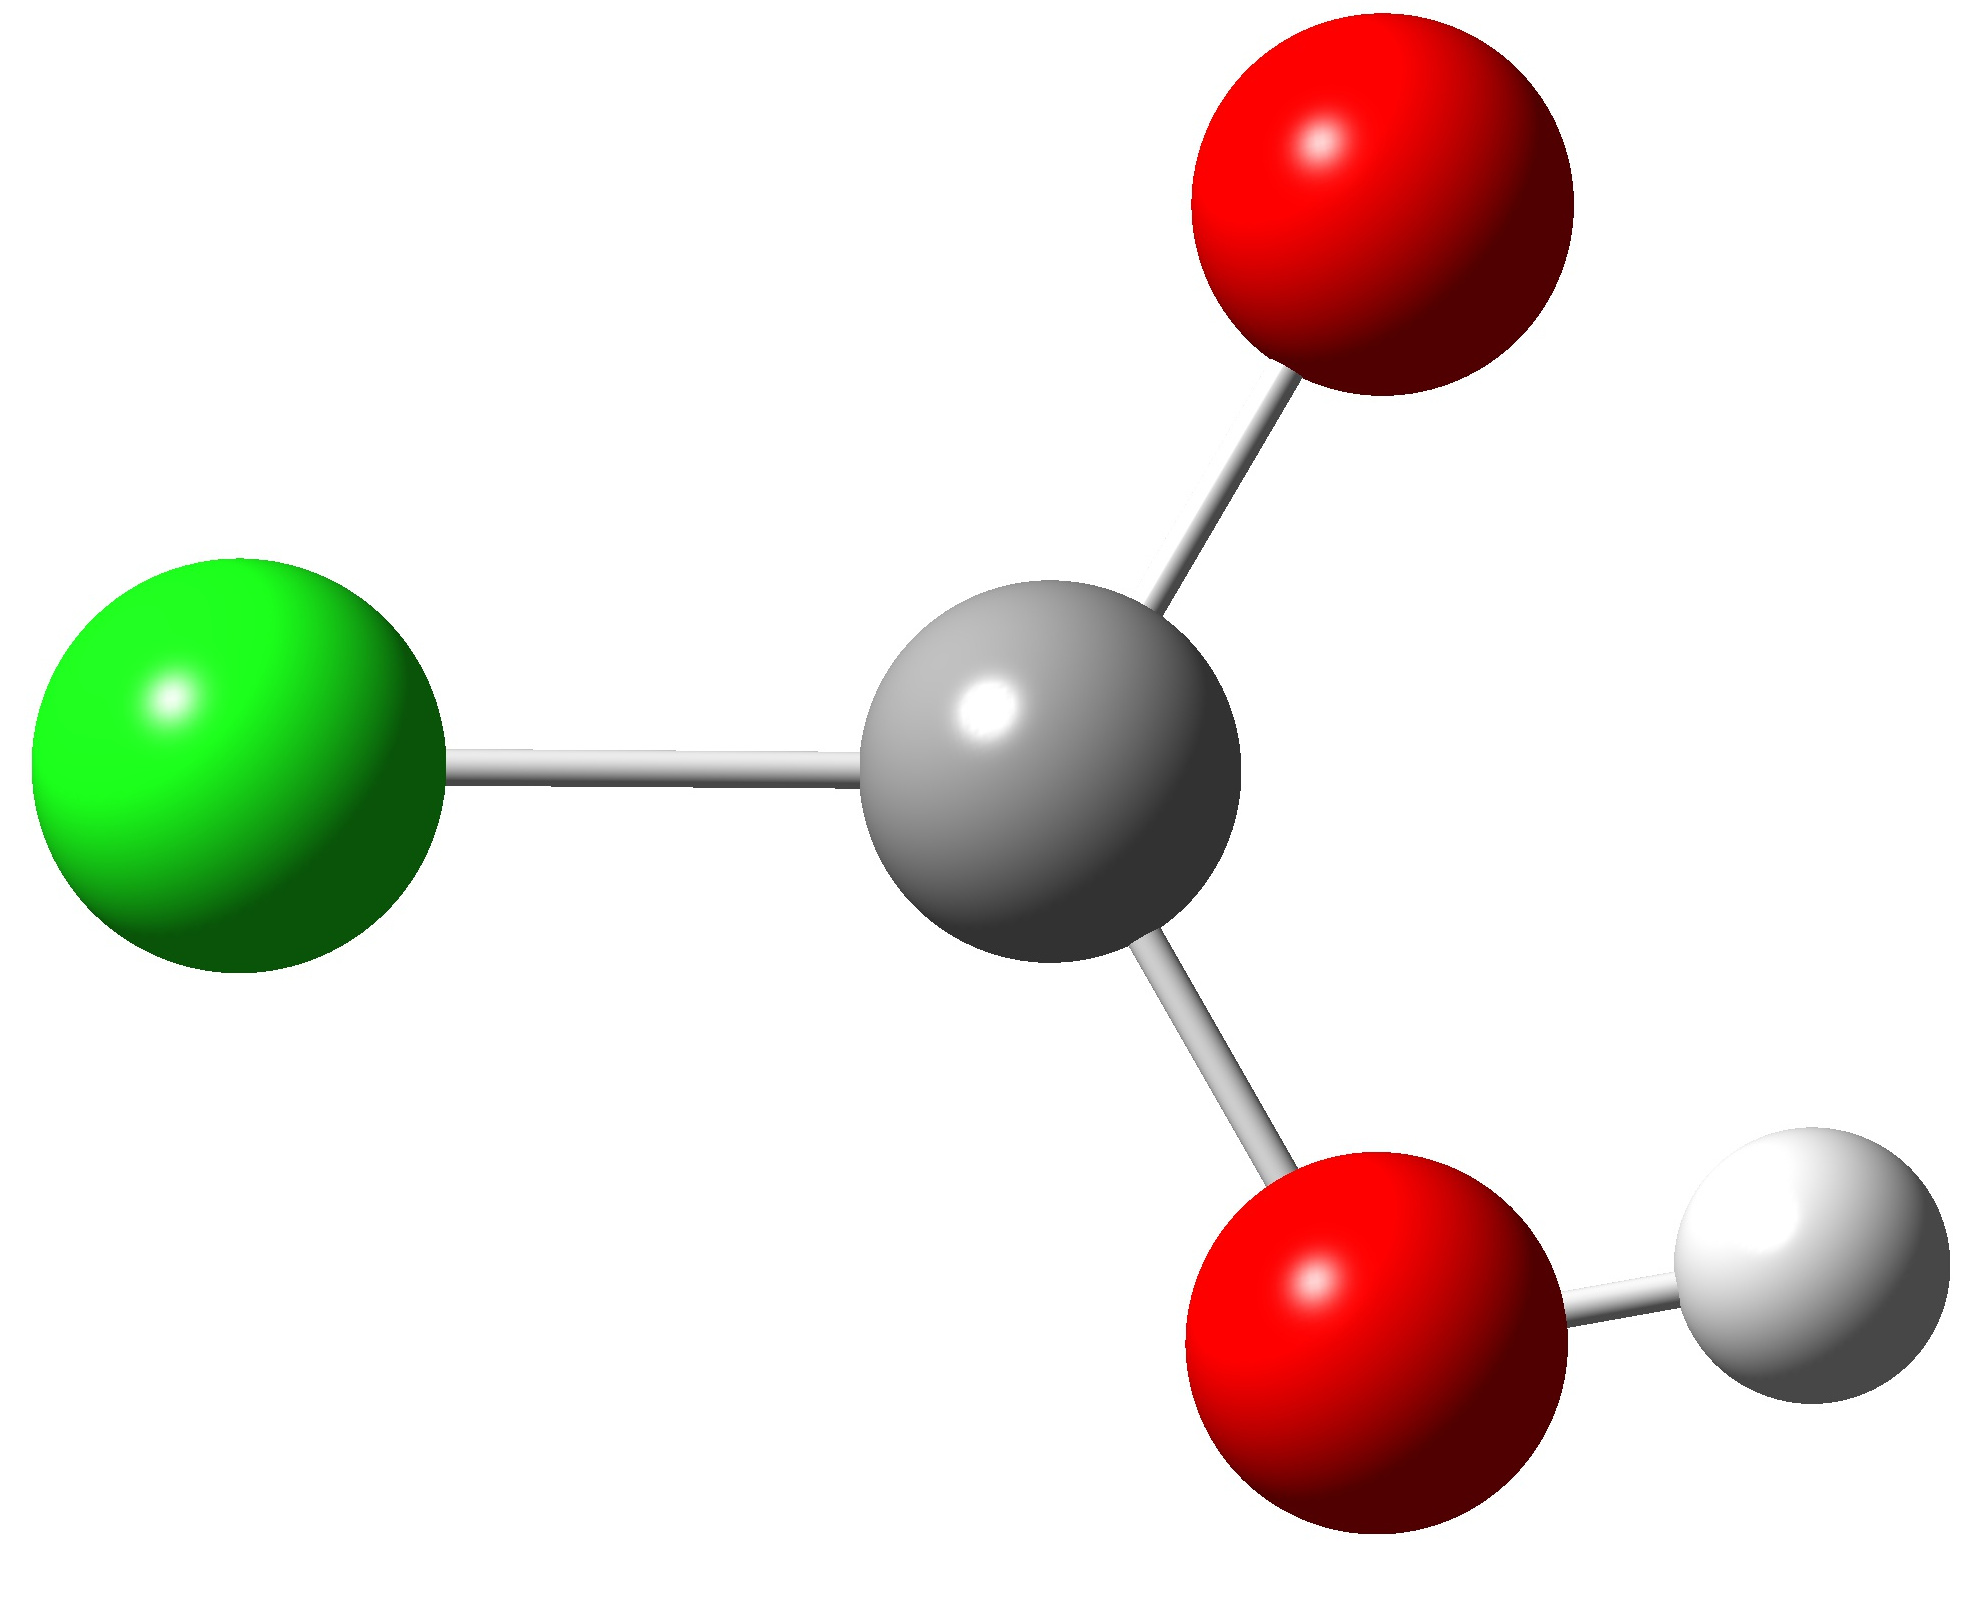
\includegraphics[scale=0.07]{carbonchloricAcid.jpg}
          \caption{Carbonochloric acid.}
        \end{minipage}
        \hfill
        \begin{minipage}[b]{0.225\textwidth}
          \centering
          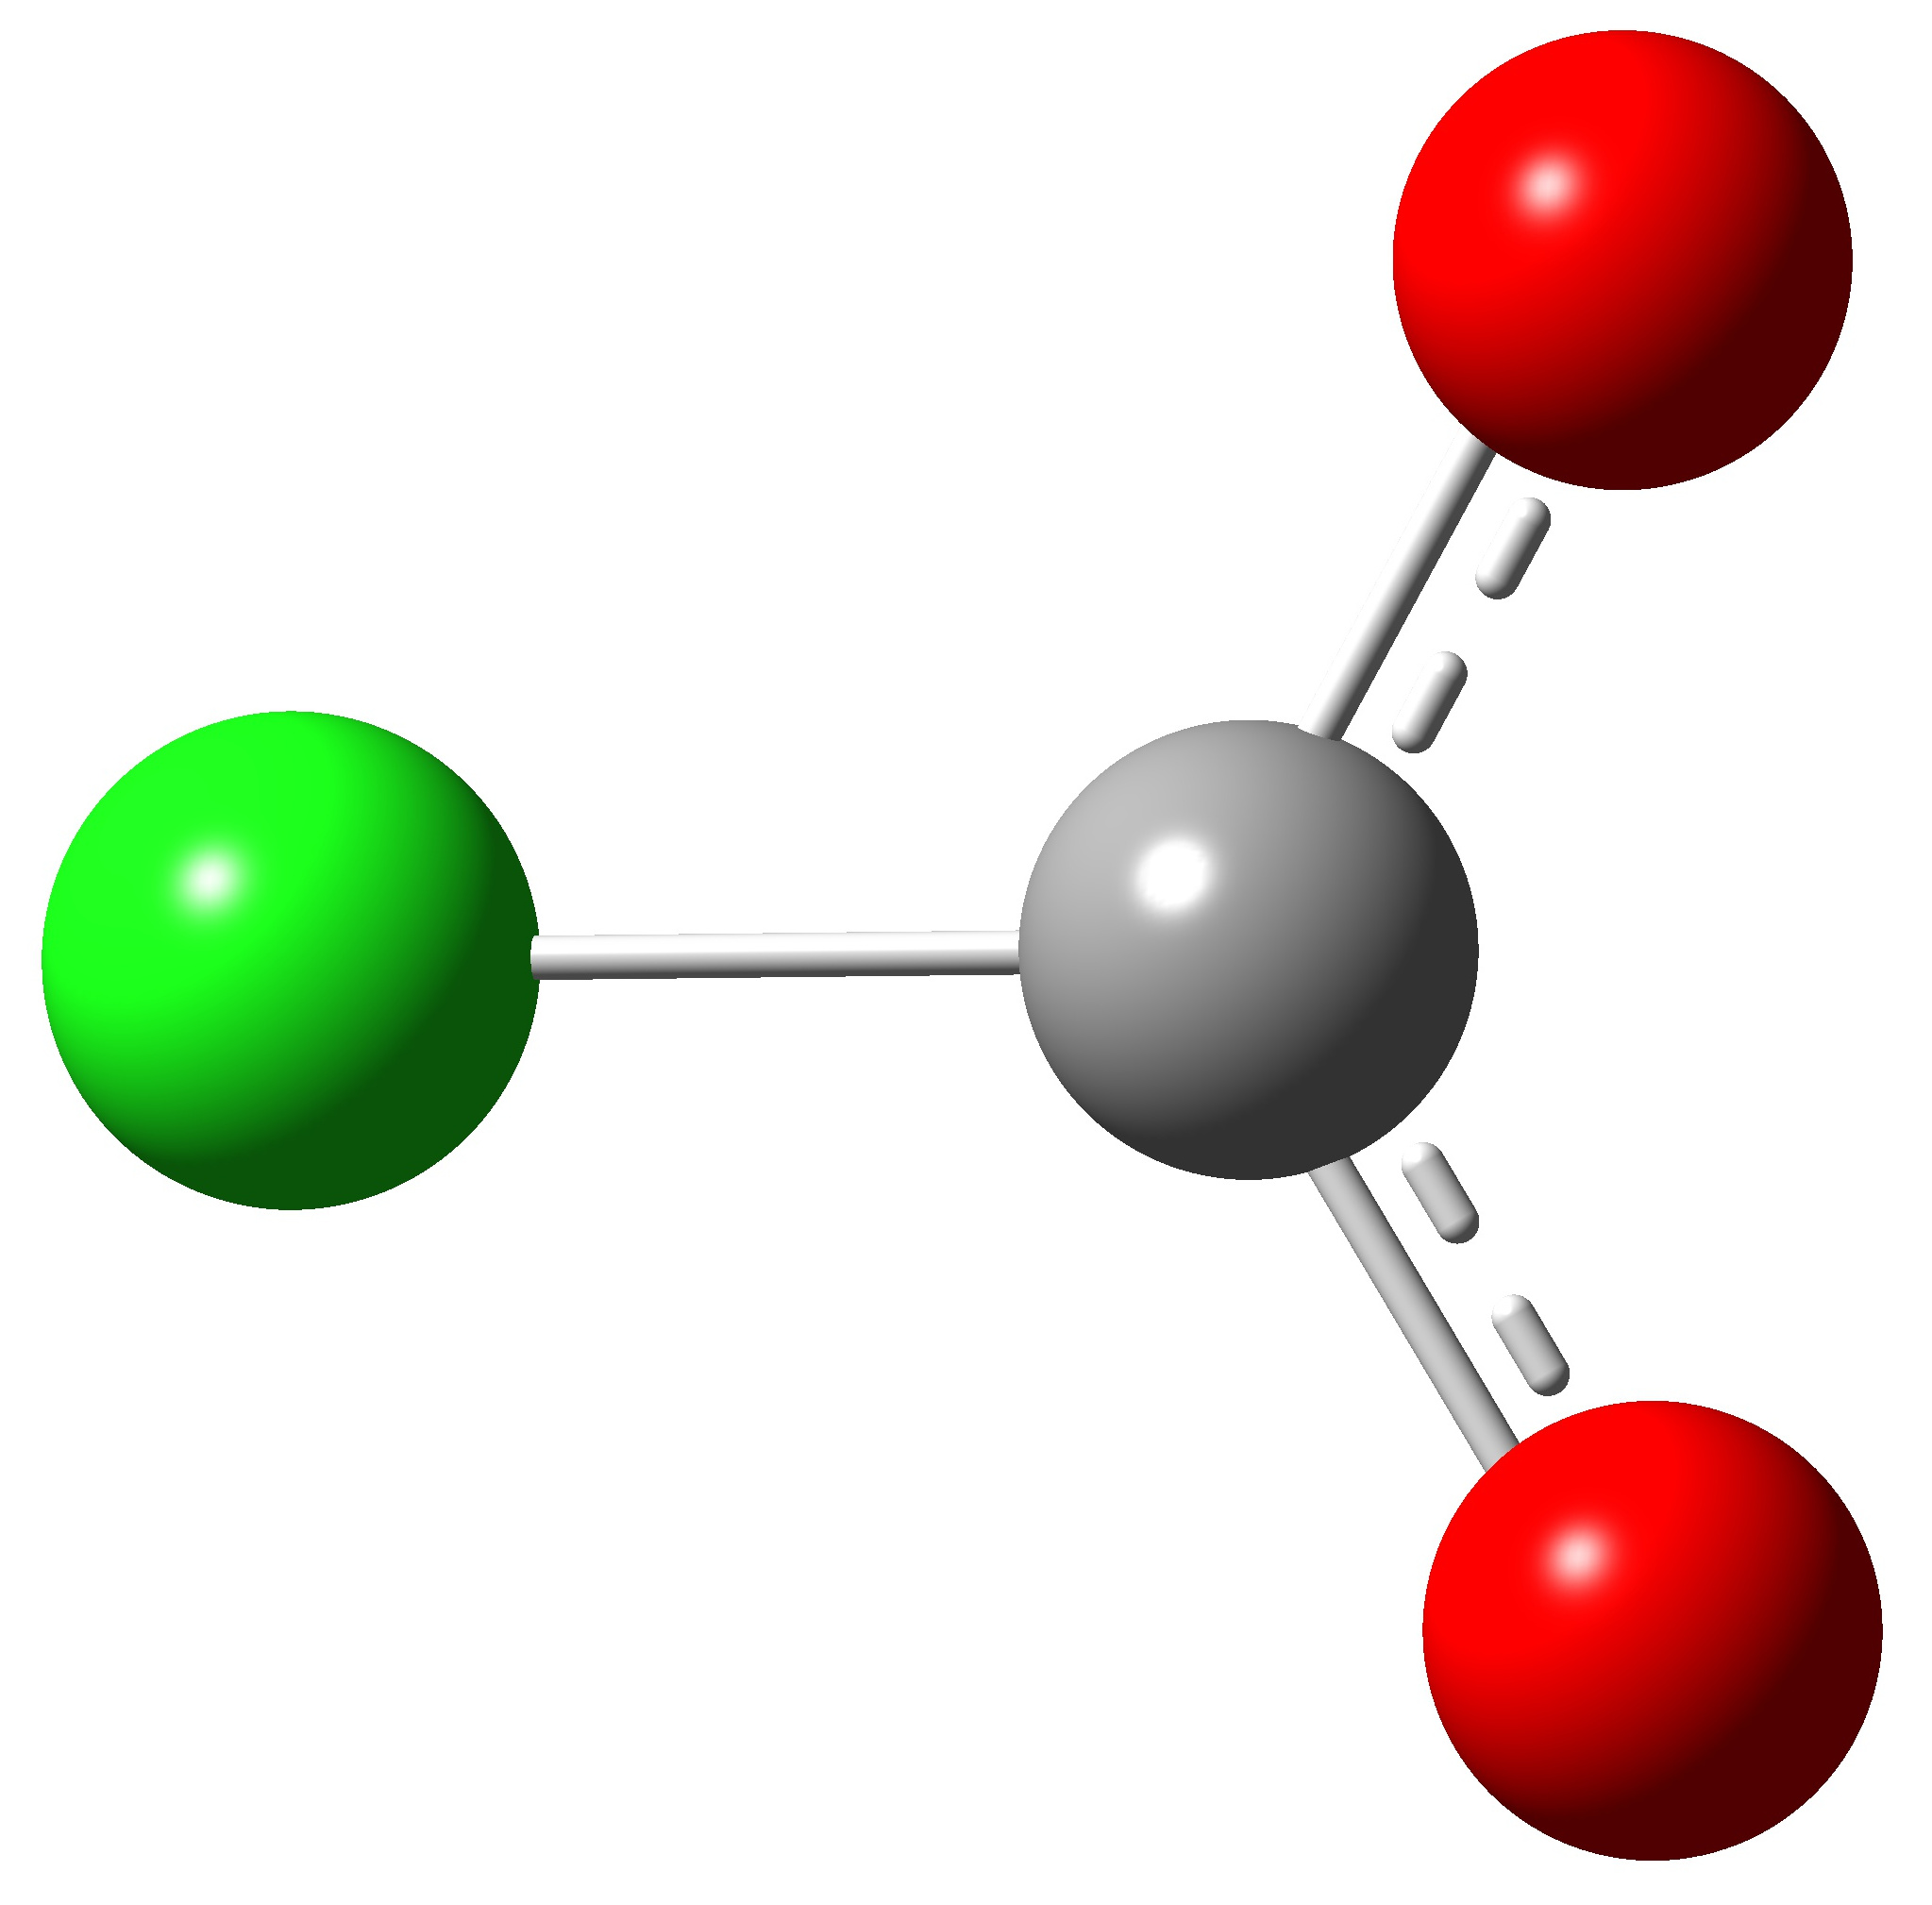
\includegraphics[scale=0.06]{carbonochloricAnion.jpg}
          \caption{Carbonochloric anion.}
        \end{minipage}
    \end{figure}
    % END FIGURE %

    \np{The calculations were performed with a laptop with an i7-8750H processor with 8GB of RAM.}

    \np{The systems shown in Figures 1-8 were run with the following settings.\n}

    \begin{lstlisting}[frame=single,gobble=10] 
            % nprocshared=4
            % mem=1500MB
            # opt freq 6-31+g(d,p) M062X scrf=smd
    \end{lstlisting}
    
    \np{\bt{NOTE:} For the supermolecule model the system is shown in figure 5 and 6 were run using the optimization obtained from systems 3 and 4, also were re-run with the following command to converge correctly \em{\# opt freq geom=check guess=check 6-31+g(d,p) scrf=smd m062x}}

    \np{For systems shown in Figures 9-12 was use the same configuration but with a basis 6-311 + G (d, p).}

    \section*{Results}
    
    \np{The computed results are shown in table 1.  }

    \titleTable{1}{Values of G in Hartree for each system.}

    \begin{center} 
        \item \import{./}{table1.tex}
    \end{center}

    \np{Were calculated the values of pka for the four acids, using the 5 methods described in the introduction, and this treatment is shown in tables 2-6 in the appendix at the end of the document.}

    \section*{Discussion}

    \np{In table 2 is observed that \bt{only consider a continuous model as SMD is not enough to get an acceptable value of pka for an acid}.}

    \np{Methods 2 and 3 give a better approximation for the value of pka, both below from 3kcal/mol this is an acceptable value for a computational calculation, but still is above 1kcal/mol, also is important to note that method 2 and 3 show similar, but the mixed model is a little better than the method 3 that consider the extrapolation of the experimental value of the proton solvation.}

    \np{Method 4 is a good approximation of the value, this is confirm the fact that the major error associated of pka calculation is from solvatation, but usign a modeling where the solvent contribution is deleted make a better calculation, and this results confirm that, because has a values with less than 1kcal/mol in the value of pka.}

    \np{For a really good value of pka the approximation of the empirical linear approximation is absolutely a good option with an error less than a 0.5kcal/mol, were tested with acetic and formic acid used in the parameterization of the straight, were tested with a basis set 6-31+g(d,p) instead of the basis used for the parameterization with 6-31++g(d,p), and we observe really good values, also were tested the propanoic acid and the results are equal of good.}

    \np{ClCOOH were totally bad calcuated any method make a correct approximation to the value, the more "nearly" was the method 5, we suppuse that this behaviur is because Cl atom is too big and is not consider correctly by the base used.}

    \np{Finally comparing table 7 is more easily see that \bt{linear approximation describe in \cite{Idaboy} is very good for linear carboxylic acids, and also the other method more general and good is method 4 that calculates pka using acid of reference and remove the solvent error, both with an error less than 1kcal/mol.}}


    %% END SECTION %%
    

    %% START REFERENCES %% 




    % DEFINE STYLE FORMAT%
    \bibliographystyle{ieeetr}
    % SPECIFY THE FILE NAMEw %
    \bibliography{references}

    %START APPENDIX (always in last page)%
    \appendix
    % CHANGE FROM X COLUMN TO ANOTHER COLUMNS EJ 2 -> 1%
    \onecolumn
    \section{Appendix}
    \begin{center}
      \item \titleTable{2}{Calculation $pk_a$ with method 1.}
      \item \import{./}{table2.tex}
      \item \titleTable{3}{Calculation $pk_a$ with method 2.}
      \item \import{./}{table3.tex}
      \item \titleTable{4}{Calculation $pk_a$ with method 3.}
      \item \import{./}{table4.tex}
      \item \titleTable{5}{Calculation $pk_a$ with method 4.}
      \item \import{./}{table5.tex}
      \item \titleTable{6}{Calculation $pk_a$ with method 5.}
      \item \import{./}{table6.tex}
      \item \titleTable{7}{Comparison of $pk_a$ calculated}
      \item \import{./}{table7.tex}
    \end{center}

    %% END REFERENCES %% 

    %%% THIS CONTENT IS IN TWO COLUMN (END) %%%

\end{document}
%%%%%%%%%%%%%%%% END DOCUMENT %%%%%%%%%%%%%%%%